%%%%%%%%%%%%%%%%%%%%%%%%%%%%%%%%%%%%%%%%%%%%%%%%%%%%%%%%%%%%%%%%%%%%%%%%%%%%%%%%
\section{Zastosowane technologie}
%%%%%%%%%%%%%%%%%%%%%%%%%%%%%%%%%%%%%%%%%%%%%%%%%%%%%%%%%%%%%%%%%%%%%%%%%%%%%%%%

Rozdział 5 zawiera opis użytych w tej pracy narzędzi. Ze względu na fakt największej styczności z platformą programistyczną .NET oraz językiem C\#, w tworzonym rozwiązaniu, skorzystano ze stosunkowo mniej popularnych zbiorów bibliotek.

Wszystkie projekty składające się na system, zostały zaimplementowane w języku programowania C\# oraz z wykorzystaniem platformy .NET w wersji 6.0.100. Jest to produkt konkurencyjny do technologii Java, jednakże działają w podobny sposób. Platforma wykorzystuje możliwości kompilowania języków programowania takich jak C\# i F\#  do dwóch wersji. Pierwsza, binarna jest dedykowana do konkretnej platformy np. Windows x64.  Drugi wariant kompiluje program do języka pośredniego, umożliwiającego  uruchomienie tworzonych rozwiązań na wszystkich platformach, na których istnieje implementacja odpowiedniej wersji środowiska uruchomieniowego .NET.

Najważniejszym dla systemów internetowych podzbiorem bibliotek platformy, są aktywne strony serwera .NET (ASP.NET Core). Dzięki swej modularności, może on służyć do stworzenia większości rodzajów aplikacji chmurowych, w sposób zapewniający im odpowiednią skalowalność oraz łatwe tworzenie testów:

\begin{itemize}
    \item Webowe interfejsy aplikacyjne (Web API) - aplikacje serwerowe, zapewniające funkcjonalność znaną ze stylów architektonicznych takich jak REST czy nowszy GraphQL. 
    \item Aplikacje chmurowe z dziedziny Internetu Rzeczy (IoT), pozwalające na łatwą manipulację danymi w systemach rozproszonych.
    \item Serwisy i mikroserwisy gRPC, stanowiące minimalistyczną i wydajną alternatywę do obarczonych większą ilością przesyłanych metadanych, webowych interfejsów aplikacyjnych.
    \item Aplikacje Model-View-Controler (MVC), wykorzystujące autorskie rozwiązanie języka znaczników Razor, jako pliki *.cshtml widoków. Razor umożliwia wykorzystanie standardowych znaczników HTML w połączeniu z logiką języka C\#. Źródłem logiki interfejsu użytkownika, są w tych aplikacjach kontrolery, odpowiedzialne również za komunikację z klasami modelu zarządzającymi danymi aplikacji.
    \item Aplikacje stron Razor (Razor Pages), w których logika związana z interfejsem użytkownika, została przeniesiona z klas kontrolerów do dedykowanych dla stron *.cshtml (opcjonalnych) plików *.cshtml.cs bedących, zwykłymi klasami języka C\#.
    \item Aplikacje Blazor, stanowiące najbardziej nowoczesny sposób tworzenia internetowych aplikacji klienckich. Platforma Blazor rozbudowuje zadania języka znaczników Razor do tworzenia całych komponentów w plikach *.razor. W odróżnieniu od architektury MVC oraz stron Razor, aplikacje te świadczą usługi aplikacji pojedynczej strony (SPA). Jest to sposób działania, znany z nowoczesnych aplikacji klienckich, tworzonych przy pomocy platform takich jak Angular, React czy Vue. Blazor odróżnia się jednak tym, że wykorzystuje w logice komponentów język C\# zamiast języka JavaScript.
\end{itemize}

Jednym z najbardziej rozpoznawalnych rozwiązań, wykorzystywanych w parze z platformą ASP.NET Core, jest dedykowane jej narzędzie mapera obiektowo-relacyjnego o nazwie Entity Framework Core (EF Core). Dzięki bardzo wygodnemu narzędziu konsolowemu platformy .NET, umożliwia on bardzo szybkie rozpoczęcie pracy na jeden z trzech sposobów, zdefiniowanych w sekcji 3.11 poświęconej narzędziom ORM.

Dodatkowym i stosunkowo niestandardowym narzędziem, w stosie technologicznym platformy .NET, jest otwarto-źródłowy menadżer pakietów Paket. Stanowi on substytut, do domyślnego narzędzia Nuget, pozwalający na większą dozę współdzielenia pakietów zewnętrznych bibliotek między projektami.

Jako silnik bazy danych, wybrano narzędzie PostgreSQL (znane również jako Postgres), będące jednym z najpopularniejszych tego typu rozwiązań na rynku, obok oprogramowania MySQL czy SQL Server. Postgres stanowi, zdecydowanie najmocniej wspierany przez społeczność akademicką, projekt otwarto-źródłowego silnika relacyjnych baz danych, skrupulatnie rozwijany i dokumentowany już od lat 90-tych XX wieku. W ostatnich latach, zyskuje nawet nowe funkcjonalności związane z przechowywaniem danych w formacie JSON, mające zapewnić mu konkurencyjność względem rozwiązań NoSQL.

Platforma NodeJS stanowi praktycznie nierozłączny element tworzenia aplikacji internetowych w dzisiejszych czasach. W przypadku projektu, opisywanego w pracy, została użyta w celu importowania pakietów JS, wykorzystywanych przez aplikację kliencką oraz sformułowania pojedynczych skryptów pomocnych w budowaniu rozwiązania.

Kolejnym elementem, składającym się na technologie wykorzystywane w projekcie, jest platforma Tailwind CSS. Jako otwarto-źródłowy produkt generujący klasy CSS, poświęcone konkretnym deklaracjom, umożliwia rezygnację z wykorzystania osobnych arkuszy stylów CSS, podnosząc czytelność komponentów projektu. Przyczynia się również do znacznego przyśpieszania powstawania prototypów aplikacji.

%%%%%%%%%%%%%%%%%%%%%%%%%%%%%%%%%%%%%%%%%%%%%%%%%%%%%%%%%%%%%%%%%%%%%%%%%%%%%%%%
\section{Projekty składające się na rozwiązanie}
%%%%%%%%%%%%%%%%%%%%%%%%%%%%%%%%%%%%%%%%%%%%%%%%%%%%%%%%%%%%%%%%%%%%%%%%%%%%%%%%

Na rozwiązanie systemu internetowego OpenOsp, tworzonego w pracy, złożyły się trzy projekty platformy .NET, dzielące między sobą konkretne zadania:

\begin{itemize}
    \item OpenOsp.Client - projekt aplikacji klienckiej wykorzystującej platfomę Blazor z modelem hostingu WebAssembly. Aplikacja zostaje pobrana w całości do pamięci przeglądarki użytkownika, w postaci binarnej i działa w pełni po stronie klienta, w sposób opisany w sekcji 3.6, poświęconej standardowi WASM. W realnym scenariuszu, umożliwia to odciążenie serwerów dostawcy usługi i m.in. oszczędność na sprzęcie.
    \item OpenOsp.Server - projekt aplikacji serwerowej odwzorowującej architekturę webowych interfejsów REST. Aplikacja wykorzystuje bibliotekę EF Core, definiując kontekst bazy danych i konfigurację poszczególnych relacji, w dedykowanych ku temu plikach. Można go uznać za główny projekt rozwiązania, ze względu na fakt serwowania usług aplikacji klienckiej przy pomocy referencji do projektu OpenOsp.Client.
    \item OpenOsp.Model - projekt biblioteki klas, składający w sobie klasy zasobów wykorzystywane przez ORM systemu, ich reprezentacje w postaci obiektów transferu danych (DTO) oraz definicje adnotacji umożliwiających łatwą walidację danych. Obydwa projekty, OpenOsp.Client i OpenOsp.Server, wykorzystują referencje do tego projektu, unikając niepotrzebnych powtórzeń w kodzie.
\end{itemize}

Przykłady implementacji funkcjonalności i opis poszczególnych części rozwiązania, zostały zawarte w kolejnych sekcjach rozdziału.

%%%%%%%%%%%%%%%%%%%%%%%%%%%%%%%%%%%%%%%%%%%%%%%%%%%%%%%%%%%%%%%%%%%%%%%%%%%%%%%%
\section{Biblioteka klas zasobów i ich reprezentacji}
%%%%%%%%%%%%%%%%%%%%%%%%%%%%%%%%%%%%%%%%%%%%%%%%%%%%%%%%%%%%%%%%%%%%%%%%%%%%%%%%

Najważniejszym katalogiem w projekcie modelu jest Models, zbierający klasy reprezentujące zasoby w aplikacji serwerowej, używane do tworzenia relacji w bazie danych. Katalogi we wszystkich projektach, segregują najczęściej poszczególne przestrzenie nazw, przykładowo OpenOsp.Model.Models dla klas zasobów.

\begin{lstlisting}[language=CSharp, caption=Przykładowa klasa zasobu, label=lst:member]
using System.Collections.Generic;
using System.ComponentModel.DataAnnotations;
using System.ComponentModel.DataAnnotations.Schema;
using OspDA = OpenOsp.Model.DataAnnotations;

namespace OpenOsp.Model.Models; 

public class Member : IHasId<int>, IOwnedBy<int> {
  [Display(Name = "First name")]
  [OspDA.Required]
  [OspDA.MaxLength(24)]
  [OspDA.Name]
  public string FirstName { get; set; }

  [Display(Name = "Last name")]
  [OspDA.Required]
  [OspDA.MaxLength(24)]
  [OspDA.Name]
  public string LastName { get; set; }

  [Display(Name = "PESEL")]
  [Column(TypeName = "char(11)")]
  [OspDA.Required]
  [OspDA.MaxLength(11)]
  [OspDA.Pesel]
  public string Pesel { get; set; }

  public virtual User User { get; set; }

  public virtual IEnumerable<ActionMember> Actions { get; set; }

  [Key] [OspDA.Required] public int Id { get; set; }

  [Display(Name = "Member owner's id")]
  [Column("OwnerId")]
  [OspDA.Required]
  public int UserId { get; set; }
}
\end{lstlisting}

Przykładowa klasa zasobu została pokazana na listingu \ref{lst:member}. Oprócz publicznych pól, z metodami dostępu, reprezentujących kolumny w tabeli, klasa posiada dwa pola wirtualne. Mogą one służyć do tworzenia zapytań pobierających z bazy danych nie tylko poszczególną encję, ale również te połączone z nią relacją jeden-do-wielu lub jeden-do-jednego. Przykładowo, w ramach zapytania wybierającego z bazy danych członka zespołu, możliwe byłoby również wybranie użytkownika będącego jego właścicielem oraz encji reprezentujących wszystkie akcje, w których brał udział.

\begin{lstlisting}[language=CSharp, caption={Interfejs implementowany przez klasy zasobu, posiadające klucz główny lub klucz złożony}, label=lst:hasId]
public interface IHasId<T>
  where T : IEquatable<T>, IComparable<T> {
  T Id { get; set; }
}

public interface IHasId<T, T2> : IHasId<T>
  where T : IEquatable<T>, IComparable<T>
  where T2 : IEquatable<T2>, IComparable<T2> {
  T2 Id2 { get; set; }
}
\end{lstlisting}

Ważną rolę w systemie pełnią interfejsy pokazane na listingach \ref{lst:hasId} oraz \ref{lst:ownedBy}. Pierwszy z nich implementowany jest przez klasy zasobów, identyfikowanych przez klucz główny lub klucz złożony. Interfejsy zastrzegają dodatkowo, że typy stosowanych kluczy, muszą implementować komparatory (interfejsy IEquatable oraz IComparable), pozwalające na porównywanie ich z wartościami tego samego typu. Dzięki funkcjonalnościom interfejsów, jest możliwe m.in tworzenie zapytań do bazy danych, przeszukujących rekordy tabeli po ich kluczach.

\begin{lstlisting}[language=CSharp, caption={Interfejs implementowany przez klasy zasobów, będących w relacji wiele-do-jednego z encją ich właściciela, identyfikowanego przez klucz główny}, label=lst:ownedBy]
public interface IOwnedBy<TUserId>
  where TUserId : IEquatable<TUserId>, IComparable<TUserId> {
  [OspDA.Required] public TUserId UserId { get; set; }
}
\end{lstlisting}

Interfejs IOwnedBy jest implementowany przez klasy zasobów, znajdujących się w relacji wiele-do-jednego ze swoim właścicielem. Ich właścicielem w systemie jest encja użytkownika, posiadająca własny klucz główny. Jednakże, dzięki zastosowaniu interfejsu, ponownie można użyć go w innych generycznych klasach systemu. W tym przypadku, będzie to automatyczne wprowadzenie klucza użytkownika do odpowiedniego atrybutu zasobu, przy jego tworzeniu oraz wykorzystanie deklarowanego klucza w mechanizmie autoryzacji per-wiersz.

Innym ważnym elementem klas zasobów są adnotacje danych, przypisane do konkretnych pól. Niektóre z nich takie jako Key i Column służą do określenia, czy dane pole klasy reprezentuje klucz główny oraz określenia nazwy i typu kolumny w tabeli. Inne można wykorzystać przy walidacji danych. Wówczas wartość pól, jest sprawdzana względem narzuconych im warunków, a w przypadku niepowodzenia, zwrócony zostanie stosowny komunikat o błędzie.

\begin{lstlisting}[language=CSharp, caption=Przykładowa klasa adnotacji danych, label=lst:name_attribute]
using System.ComponentModel.DataAnnotations;

namespace OpenOsp.Model.DataAnnotations; 

public class NameAttribute : RegularExpressionAttribute {
  public NameAttribute() : base(@"^[\p{L} \.\-]+$") {
    ErrorMessage = @"{0} is not a valid name";
  }
}
\end{lstlisting}

Przykładowo, na listingu \ref{lst:name_attribute} przedstawiono adnotację danych NameAttribute, służącą walidacji pól łańcuchów znaków, przy pomocy zdefiniowanego wyrażenia regularnego (regex). Wszystkie zdefiniowane podczas tworzenia systemu adnotacje danych, zostały zawarte w katalogu DataAnnotations i poświęconej im przestrzeni nazw OpenOsp.Model.DataAnnotations. 

W przypadku nieudanej walidacji, zostanie użyty komunikat o błędzie zdefiniowany w konstruktorze. W miejsce znacznika "{0}" wstawiona zostanie wizualna nazwa pola. Nazwa pola może zostać ustawiona ręcznie przy pomocy adnotacji Display, tak jak zostało to pokazane na listingu \ref{lst:member}.

Ważnym elementem w strukturze projektu jest katalog Dtos, zrzeszający pod jedną przestrzenią nazw, obiekty transferu danych będące m.in. reprezentacjami zasobów w systemie. Zawiera w sobie zarówno klasy obiektów, jak i klasy tzw. maperów tworzących obiekty zasobów, z obiektów ich reprezentacji i na odwrót.

\begin{lstlisting}[language=CSharp, caption={Przykładowa klasa obiektu transferu danych, stanowiąca reprezentację odczytu zasobu}, label=lst:member_read_dto]
using System.ComponentModel.DataAnnotations;
using OspDA = OpenOsp.Model.DataAnnotations;

namespace OpenOsp.Model.Dtos; 

public class MemberReadDto {
  [OspDA.Required] public int Id { get; set; }

  [Display(Name = "First name")]
  [OspDA.Required]
  [OspDA.MaxLength(24)]
  [OspDA.Name]
  public string FirstName { get; set; }

  [Display(Name = "Last name")]
  [OspDA.Required]
  [OspDA.MaxLength(24)]
  [OspDA.Name]
  public string LastName { get; set; }

  [Display(Name = "PESEL")]
  [OspDA.Required]
  [OspDA.Pesel]
  public string Pesel { get; set; }
}
\end{lstlisting}

\begin{lstlisting}[language=CSharp, caption={Przykładowa klasa obiektu transferu danych, stanowiąca reprezentację aktualizacji zasobu}, label=lst:member_update_dto]
using System.ComponentModel.DataAnnotations;
using OspDA = OpenOsp.Model.DataAnnotations;

namespace OpenOsp.Model.Dtos; 

public class MemberUpdateDto {
  [Display(Name = "First name")]
  [OspDA.Required]
  [OspDA.MaxLength(24)]
  [OspDA.Name]
  public string FirstName { get; set; }

  [Display(Name = "Last name")]
  [OspDA.Required]
  [OspDA.MaxLength(24)]
  [OspDA.Name]
  public string LastName { get; set; }

  [Display(Name = "PESEL")]
  [OspDA.Required]
  [OspDA.Pesel]
  public string Pesel { get; set; }
}
\end{lstlisting}

Klasy transferu danych, najczęściej definiuje się dla operacji tworzenia, odczytu, aktualizacji i usuwania zasobu (CRUD). Jako przykład na listingach \ref{lst:member_read_dto} i \ref{lst:member_update_dto} pokazano klasy poświęcone odczytowi i aktualizacji zasobów członka zespołu. Większość z ich pól powtarza się, jednakże operacja odczytu przekazuje klientowi również klucz główny danej encji. 

Operacja aktualizacji zakłada wcześniejszy odczyt i uzyskanie potrzebnego do przeprowadzenia identyfikatora (ścieżki) zasobu. Podział odpowiedzialności na kilka prostych klas, zapewnia łatwość modyfikacji reprezentacji zasobów oraz oszczędność na przesyle danych.

\begin{lstlisting}[language=CSharp, caption=Przykładowa klasa mapera klas zasobów na klasy jego reprezentacji i na odwrót, label=lst:member_dto_mapper]
using OpenOsp.Model.Models;

namespace OpenOsp.Model.Dtos.Mappers; 

public class MemberDtoMapper : IDtoMapper<Member, MemberCreateDto, MemberReadDto, MemberUpdateDto> {
  public Member MapCreate(MemberCreateDto dto) {
    return new Member {FirstName = dto.FirstName, LastName = dto.LastName, Pesel = dto.Pesel};
  }

  public MemberUpdateDto MapPatch(Member entity) {
    return new MemberUpdateDto {FirstName = entity.FirstName, LastName = entity.LastName, Pesel = entity.Pesel};
  }

  public MemberReadDto MapRead(Member entity) {
    return new MemberReadDto {
      FirstName = entity.FirstName, Id = entity.Id, LastName = entity.LastName, Pesel = entity.Pesel
    };
  }

  public Member MapUpdate(MemberUpdateDto dto, Member entity) {
    entity.FirstName = dto.FirstName;
    entity.LastName = dto.LastName;
    entity.Pesel = dto.Pesel;
    return entity;
  }
}
\end{lstlisting}

W celu uniknięcia niepotrzebnych powtórzeń, w kodzie kontrolerów aplikacji serwerowej, zaleca się definiować pomocnicze klasy maperów dla zasobów i ich reprezentacji. Maper dla klasy członka zespołu oraz wszystkich jego reprezentacji został przedstawiony na listingu \ref{lst:member_dto_mapper}.

%%%%%%%%%%%%%%%%%%%%%%%%%%%%%%%%%%%%%%%%%%%%%%%%%%%%%%%%%%%%%%%%%%%%%%%%%%%%%%%%
\section{Punkt startowy systemu}
%%%%%%%%%%%%%%%%%%%%%%%%%%%%%%%%%%%%%%%%%%%%%%%%%%%%%%%%%%%%%%%%%%%%%%%%%%%%%%%%

Aplikacja serwerowa jest najbardziej złożonym z projektów w całym rozwiązaniu. Na jej działanie składa się wykorzystanie kodu kilkunastu bibliotek (listing \ref{lst:paket_server}), umożliwiających tworzenie kompleksowych systemów nawet w niewielkich zespołach.

\begin{lstlisting}[language=CSharp, caption=Plik menadżera pakietów stanowiący spis referencji do zewnętrznych bibliotek .NET w aplikacji serwerowej, label=lst:paket_server]
Microsoft.AspNetCore.Authentication
Microsoft.AspNetCore.Authentication.JwtBearer
Microsoft.AspNetCore.Components.WebAssembly.Server
Microsoft.AspNetCore.Cors
Microsoft.AspNetCore.Identity
Microsoft.AspNetCore.Identity.EntityFrameworkCore
Microsoft.AspNetCore.JsonPatch
Microsoft.AspNetCore.Mvc.NewtonsoftJson
Microsoft.EntityFrameworkCore.Design
Microsoft.EntityFrameworkCore.Relational
Microsoft.EntityFrameworkCore.Tools
Microsoft.Extensions.Configuration.Json
Microsoft.Extensions.Identity.Stores
Microsoft.IdentityModel.Tokens
Npgsql.EntityFrameworkCore.PostgreSQL
Swashbuckle.AspNetCore
\end{lstlisting}

Budowanie i rozpoczęcie świadczenia usług aplikacji serwerowej, podobnie jak większości aplikacji .NET, rozpoczyna się w metodzie Main() klasy Program, która okazuje się być wyjątkowo minimalistyczna. Jest tak ze względu na przerzucenie odpowiedzialności za konfiguracje serwisów oraz kontrolerów aplikacji na klasę Startup, typową dla aplikacji platformy ASP.NET Core.

\begin{lstlisting}[language=CSharp, caption=Klasa Program w aplikacji serwerowej rozwiązania, label=lst:program_server]
using Microsoft.AspNetCore.Hosting;
using Microsoft.Extensions.Hosting;

namespace OpenOsp.Server; 

public class Program {
  public static void Main(string[] args) {
    CreateHostBuilder(args).Build().Run();
  }

  public static IHostBuilder CreateHostBuilder(string[] args) {
    return Host.CreateDefaultBuilder(args)
      .ConfigureWebHostDefaults(webBuilder => {
        webBuilder.UseStartup<Startup>();
      });
  }
}
\end{lstlisting}

Klasa Startup (listing \ref{lst:startup_server}) składa się z dwóch głównych metod, wykorzystujących pochodną wzorca projektowego "budowniczy" (builder), na potrzeby procesu konfiguracji. Pierwsza z nich, ConfigureServices() wywołuje metody interfejsu IServiceContainer, aby dodawać i konfigurować serwisy w kontenerze IoC. Druga metoda klasy to Configure(), definiująca  zachowania interfejsu aplikacji względem żądań HTTP, poprzez wywołania metod interfejsu IApplicationBuilder. 

Przykładowo, pozwala ona zastosować przekierowania do zaszyfrowanej wersji interfejsu (HTTPS), dodać autoryzację dostępu do zasobów lub np. serwować pliki statyczne aplikacji klienckiej z innego projektu. 

\begin{lstlisting}[language=CSharp, caption=Elementy klasy Startup w aplikcji serwerowej, label=lst:startup_server]
public class Startup {
  private readonly IWebHostEnvironment _env;

  public Startup(
    IConfiguration configuration,
    IWebHostEnvironment env) {
    Configuration = configuration;
    _env = env;
  }

  public IConfiguration Configuration { get; }

  public void ConfigureServices(IServiceCollection services) {
    ...
  }

  public void Configure(IApplicationBuilder app) {
    ...
  }
}
\end{lstlisting}

Klasa korzysta również z serwisów IConfiguration i IWebHostEnvironment, wstrzykiwanych przez konstruktor, na etapie budowania aplikacji. Pierwszy z nich, umożliwia dostęp do zawartości pliku appsettings.json, opisującego ustawienia aplikacji. Drugi, daje dostęp do informacji o zmiennych środowiskowych, zastosowanych na etapie budowania projektu.

%%%%%%%%%%%%%%%%%%%%%%%%%%%%%%%%%%%%%%%%%%%%%%%%%%%%%%%%%%%%%%%%%%%%%%%%%%%%%%%%
\section{Zastrzyki zależności w aplikacjach ASP.NET Core}
%%%%%%%%%%%%%%%%%%%%%%%%%%%%%%%%%%%%%%%%%%%%%%%%%%%%%%%%%%%%%%%%%%%%%%%%%%%%%%%%

Zastrzyk zależności jest jednym z najpopularniejszych wzorców projektowych, wykorzystywanych we współcześnie tworzonych aplikacjach. U jego podstawy, leży zasada luźnego powiązania między komponentami programu. W odróżnieniu od powiązań twardych, w przypadku wprowadzenia zmian w klasie serwisu, od której zależna jest tzw. klasa klienta, nie są potrzebne zmiany w klasie klienta.

\begin{figure}[!htbp] 
    \centering
    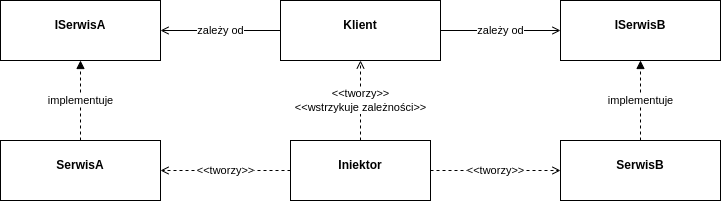
\includegraphics[width=\textwidth]{img/chapter5/dependency_injection.png}
    \caption{Wizualizacja wzorca projektowego zastrzyków zależności w postaci diagramu klas}
    \label{fig:dependency_injection}
\end{figure}

Same zastrzyki są procesem tworzenia i przekazywania obiektów serwisów, do zależnych od nich klientów, przy pomocy obiektu Iniektora. Na rys. \ref{fig:dependency_injection} przedstawiono prostą wizualizację zastosowania wzorca. Zadaniem takiego rozwiązania jest zmniejszenie do minimum, ilości twardych powiązań klas w projektach programów. Czyni je to bardziej skalowalnymi, łatwiejszymi w testowaniu oraz dokumentowaniu i obiektywnie lepszymi programistyczne rozwiązaniami (np. zachowanie zasady pojedynczej odpowiedzialności komponentów).

Zastrzyk zależności może nastąpić na trzy różne sposoby. Najpopularniejszą z metod, jest przekazywanie tworzonego obiektu przez interfejs, będący argumentem konstruktora obiektu klienta. Pozostałe dwie to: przekazanie obiektu przy pomocy metody dostępowej pola C\# lub przez argument dowolnej innej metody klasy. Najwięcej zalet, posiada metoda wykorzystująca konstruktor, która pozwala uniknąć odwołań do referencji serwisów wskazujących na adres zerowy, ustawiając ich adres przy tworzeniu obiektu klienta.

Kolejnym ważnym elementem, jest kontener odwróconej kontroli (IoC), umożliwiający automatyzację procesu wstrzykiwania zależności w aplikacjach. W przypadku platformy ASP.NET Core, podstawowy kontener IoC jest zawarty w jej kodzie, umożliwiając łatwe rozpoczęcie pracy z tym wzorcem. Przykłady jego użycia można znaleźć w metodzie ConfigureServices() klasy Startup (patrz listing \ref{lst:startup_server}). Obiekt implementujący interfejs IServiceCollection, przekazywany jest do niej jako argument i umożliwia ręczną konfigurację zależności, wykorzystywanych przez automatyczny iniektor platformy.

\begin{lstlisting}[language=CSharp, caption=Fragment ciała metody Startup.ConfigureServices() poświęcony konfiguracji przekierowania do strony w wersji HTTPS, label=lst:startup_configureServices_basics]
services.AddHttpsRedirection(options => {
  options.RedirectStatusCode = (int)HttpStatusCode.PermanentRedirect;
  options.HttpsPort = _env.IsDevelopment() ? 5001 : 443;
});
\end{lstlisting}

Wiele ze wstrzykiwanych w ten sposób serwisów, konfiguruje się wykorzystując metody rozszerzające kolekcję serwisów, zdefiniowane w poszczególnych bibliotekach. Przykładowo, fragment z listingu \ref{lst:startup_configureServices_basics} wywołuje metodę rejestrującą serwis obsługujący przekierowanie klienta na stronę w wersji HTTPS. Jednakże, chcąc zarejestrować serwisy zdefiniowane przez użytkownika, można posłużyć się trzema dostępnymi metodami generycznymi, określającymi cykl życia danego serwisu:

\begin{itemize}
    \item AddSingleton() - obiekt serwisu zarejestrowanego przy pomocy metody singleton, zostaje utworzony tylko raz, przy pierwszym wstrzyknięciu i jest współdzielony między wszystkimi zależnymi od niego klientami, aż do końca życia aplikacji. Wykorzystanie wzorca projektowego singleton w ten sposób, zapewnia również implementację, potencjalnie lepiej przystosowaną do wielowątkowości.
    \item AddScoped() - rejestrując serwisy ograniczone zakresem żądania, zapewniamy, że tworzone obiekty zostają użyte tylko w ramach konkretnego żądania HTTP. Obiekty są tworzone na początku konkretnego żądania HTTP i są współdzielone między wszystkimi klientami, obsługującymi to żądanie.
    \item AddTransient() - obiekty serwisów przemijających, są tworzone ekskluzywnie dla każdego klienta, gdy są potrzebne. Nigdy nie są współdzielone między różnymi klientami.
\end{itemize}

Fragmenty kodu rejestrującego serwisy, powiązane z poszczególnymi zadaniami, zostały przytoczone w odpowiednich sekcjach dalszej części pracy. 

%%%%%%%%%%%%%%%%%%%%%%%%%%%%%%%%%%%%%%%%%%%%%%%%%%%%%%%%%%%%%%%%%%%%%%%%%%%%%%%%
\section{Kontekst bazy danych i migracje Entity Framework Core}
%%%%%%%%%%%%%%%%%%%%%%%%%%%%%%%%%%%%%%%%%%%%%%%%%%%%%%%%%%%%%%%%%%%%%%%%%%%%%%%%

Kolejnym tematem jest sposób połączenia aplikacji z bazą danych. Aplikacja wykorzystuje ORM EF Core dla, którego najważniejszą klasą jest kontekst bazy danych.

\begin{lstlisting}[language=CSharp, caption=Klasa kontekstu bazy danych, label=lst:appDbContext]
public class AppDbContext : IdentityUserContext<User, int> {
  private readonly int _userId;

  public AppDbContext() { }

  public AppDbContext(DbContextOptions<AppDbContext> options) : base(options) { }

  public AppDbContext(DbContextOptions<AppDbContext> options, 
      IUserClaimsService<int> userClaims) : base(options) {
    _userId = userClaims.UserId;
  }

  public virtual DbSet<Action> Actions { get; set; }
  public virtual DbSet<ActionEquipment> ActionEquipment { get; set; }
  public virtual DbSet<ActionMember> ActionMembers { get; set; }
  public virtual DbSet<Equipment> Equipment { get; set; }
  public virtual DbSet<Member> Members { get; set; }
  public override DbSet<User> Users { get; set; }

  protected override void OnModelCreating(ModelBuilder builder) {
    base.OnModelCreating(builder);
    ...
  }

  public override async Task<int> SaveChangesAsync(CancellationToken cancellationToken = default) {
    ...
  }
}
\end{lstlisting}

Na listingu \ref{lst:appDbContext} ukazano najważniejszą część klasy kontekstu, w której publiczne pola o generycznych typach DbSet, reprezentują poszczególne tabele (relacje) zasobów w bazie danych. Oprócz konstruktorów, umożliwiających skonfigurowanie połączenia z bazą danych, kontekst posiada zasłoniętą metodę OnModelCreating(), której ciało umożliwia zastosowanie dodatkowej konfiguracji na relacji w bazie danych.

\begin{lstlisting}[language=CSharp, caption=Przykładowa klasa konfiguracyjna relacji w bazie danych wykorzystująca interfejs biegły Entity Framework Core, label=lst:member_config]
internal class MemberConfiguration : IEntityConfiguration {
  public void AddConfiguration(ModelBuilder builder) {
    builder.Entity<Member>(entity => {
      entity.HasKey(e => e.Id);
      entity.Property(e => e.Id)
        .IsRequired()
        .ValueGeneratedOnAdd();
      entity.Property(e => e.FirstName)
        .IsRequired()
        .HasMaxLength(24);
      entity.Property(e => e.LastName)
        .IsRequired()
        .HasMaxLength(24);
      entity.Property(e => e.Pesel)
        .HasColumnType("char(11)")
        .IsRequired()
        .HasMaxLength(11);
      entity.Property(e => e.UserId)
        .HasColumnName("OwnerId")
        .IsRequired();
      entity.HasOne(e => e.User)
        .WithMany(e => e.Members)
        .OnDelete(DeleteBehavior.NoAction);
      entity.HasMany(e => e.Actions)
        .WithOne(e => e.Member)
        .OnDelete(DeleteBehavior.Cascade);
    });
  }

  public void SeedData(ModelBuilder builder) {
    ...
  }
}
\end{lstlisting}

Konfigurację poszczególnych zasobów podzielono na klasy, zawierające dwie metody. Metoda AddConfiguration() służy wprowadzeniu ograniczeń dla atrybutów zasobu oraz określaniu jego relacji jeden-do-wielu, wiele-do-jednego oraz jeden-do-jednego. Druga metoda, SeedData() służy do utworzenia encji, automatycznie wpisanych do tabeli podczas tworzenia bazy.

Przykładowa konfiguracja, zasobu członka zespołu z listingu \ref{lst:member_config} określa typ kolumny Pesel jako char(11), czyniąc ją jednocześnie wartością wymaganą i ograniczając maksymalną długość jej wartości do 11 znaków. Na budowniczym encji, użyto metod definiujących jej relację wiele-do-jednego z właścicielem encji członka zespołu oraz relacji jeden-do-wielu z akcjami, w których wziął udział.

\begin{lstlisting}[language=CSharp, caption=Fragment metody AppDbContext.OnModelCreating() poświęcony klasom konfiguracyjnym encji, label=lst:onModelCreating_configs]
IEnumerable<IEntityConfiguration> entityConfigurations = new List<IEntityConfiguration> {
  new ActionConfiguration(),
  new ActionEquipmentConfiguration(),
  new ActionMemberConfiguration(),
  new EquipmentConfiguration(),
  new MemberConfiguration(),
  new UserConfiguration()
};
foreach (var entityConfiguration in entityConfigurations) {
  entityConfiguration.AddConfiguration(builder);
  entityConfiguration.SeedData(builder);
}
\end{lstlisting}

Konfiguracje można wykorzystać w metodzie OnModelCreating() kontekstu. Część z zastosowanych w nich opcji jest redundantne, względem adnotacji danych w klasie zasobu. Jednakże, niektóre ograniczenia są możliwe tylko dzięki biegłemu interfejsowi (Fluent API) EF Core. Przykładem takich ustawień, jest zastosowanie klucza złożonego (składającego się z więcej niż jednego atrybutu) oraz zastosowanie ochrony per-wiersz, opisanej w sekcji poświęconej użytkownikom systemu.

\begin{lstlisting}[language=CSharp, caption=Rejestracja kontekstu bazy danych jako serwis w metodzie Startup.ConfigureServices(), label=lst:config_appDbContext]
services.AddDbContext<AppDbContext>(options => {
  options.UseNpgsql(
      Configuration.GetConnectionString("PostgreSql"),
      builder => builder.EnableRetryOnFailure(5, TimeSpan.FromSeconds(10), null)
    )
    .EnableSensitiveDataLogging(false);
});
\end{lstlisting}

W celu zarejestrowania kontekstu bazy danych, jako serwisu do wstrzykiwania w zależnych od niego klientach, należy dodać fragment kodu widoczny na listingu \ref{lst:config_appDbContext} do ciała funkcji Startup.ConfigureServices(). 

\begin{lstlisting}[language=JavaScript, caption=Fragment pliku konfiguracyjnego appsettings.json zawierający łańcuch połączenia z bazą danych, label=lst:appsettings_conStr]
"ConnectionStrings": {
  "PostgreSql": "Host=ec2-18-202-156-92.eu-west-1.compute.amazonaws.com;Port=5432;Database=d92n4e7hua6lht;Username=lundqzkmrjkhry;Password=1e089e898b0ee3a9a3863e3be4921f37ed691a8a40dc2c02d876c382934d29c8"
 },
\end{lstlisting}

Wstrzyknięty na etapie budowania, serwis IConfiguration umożliwia uzyskanie łańcucha połączenia z bazą, przy pomocy dedykowanej metody serwisu konfiguracyjnego GetConnectionString().

Ostatnią częścią, klas odpowiedzialnych za interakcje z bazą danych, są migracje. Po zarejestrowaniu kontekstu bazy jako serwis, dostępne staje się narzędzie konsolowe dotnet-ef. Umożliwia tworzenie migracji modelu oraz aktualizowanie struktury bazy danych.

\begin{lstlisting}[language=CSharp, caption=Przykładowa klasa migracji Entity Framework Core, label=lst:migration]
public partial class Members_Pesel_TypeFromVarcharToChar : Migration
{
    protected override void Up(MigrationBuilder migrationBuilder)
    {
        migrationBuilder.AlterColumn<string>(
            name: "Pesel",
            table: "Members",
            type: "char(11)",
            maxLength: 11,
            nullable: false,
            oldClrType: typeof(string),
            oldType: "varchar(11)",
            oldMaxLength: 11);
    }

    protected override void Down(MigrationBuilder migrationBuilder)
    {
        migrationBuilder.AlterColumn<string>(
            name: "Pesel",
            table: "Members",
            type: "varchar(11)",
            maxLength: 11,
            nullable: false,
            oldClrType: typeof(string),
            oldType: "char(11)",
            oldMaxLength: 11);
    }
}
\end{lstlisting}

Przykładowa klasa migracji (a właściwie jej czytelna dla ludzi część), utworzona na etapie optymalizacji zapytań do bazy danych, została pokazana na listingu \ref{lst:migration}. Tworząc ją, zamieniono typ kolumny atrybutu Pesel w tabeli członków zespołu, z varchar(11) na char(11). Pozwala to na oszczędność miejsca w bazie oraz zoptymalizowanie procesu wyboru krotek encji.

Metoda Up() migracji wskazuje, jakie zapytania powinny zostać wykonane przez ORM, aby zastosować zmiany, dokonane w kodzie modelu bazy (zasobów i kontekstu). Metoda Down() jest stosowana w przypadku cofania tych zmian. Jednakże, jak zostało opisane w sekcji rozdziału teoretycznego poświęconemu narzędziom ORM, zawsze należy upewnić się czy zastosowanie lub wycofanie danej migracji nie wiąże się z ryzykiem utraty danych.

%%%%%%%%%%%%%%%%%%%%%%%%%%%%%%%%%%%%%%%%%%%%%%%%%%%%%%%%%%%%%%%%%%%%%%%%%%%%%%%%
\section{Warstwy interfejsu REST}
%%%%%%%%%%%%%%%%%%%%%%%%%%%%%%%%%%%%%%%%%%%%%%%%%%%%%%%%%%%%%%%%%%%%%%%%%%%%%%%%

W tej sekcji opisano trzy rodzaje klas składających się na funkcjonalności interfejsu REST aplikacji serwerowej.

%%%%%%%%%%%%%%%%%%%%%%%%%%%%%%%%%%%%%%%%%%%%%%%%%%%%%%%%%%%%%%%%%%%%%%%%%%%%%%%%
\subsection{Repozytoria}
%%%%%%%%%%%%%%%%%%%%%%%%%%%%%%%%%%%%%%%%%%%%%%%%%%%%%%%%%%%%%%%%%%%%%%%%%%%%%%%%

\begin{lstlisting}[language=CSharp, caption=Generyczna klasa podstawowego repozytorium zasobów, label=lst:repository]
public class Repository<T> : IRepository<T> where T : class {
  private readonly AppDbContext _context;

  public Repository(AppDbContext context) {
    _context = context;
  }

  public void Create(T entity) {
    _context.Add(entity);
  }

  public void Update(T entity) {
    _context.Update(entity);
  }

  public void Delete(T entity) {
    _context.Remove(entity);
  }

  public virtual IQueryable<T> ReadAll() {
    return _context.Set<T>();
  }

  public IQueryable<T> ReadAll(PaginationFilter pagination) {
    return ReadAll().Skip((pagination.PageIndex - 1) * pagination.PageSize)
      .Take(pagination.PageSize);
  }

  public async Task<int> SaveChangesAsync() {
    return await _context.SaveChangesAsync();
  }
}
\end{lstlisting}

Repozytoria są klasami najbliższymi do warstwy danych. Odpowiadają za tworzenie zapytań do bazy danych, wykorzystując tzw. biegłe metody biblioteki LINQ na polach wstrzykniętego obiektu kontekstu bazy. W ramach metod zdefiniowanych w repozytoriach, nie dochodzi do przesłania zapytań, do silnika bazy danych. Dzieje się to dopiero w klasach serwisów, określających, jaką strukturę danych należy utworzyć ze zwróconych rekordów.

\begin{lstlisting}[language=CSharp, caption=Generyczne klasy repozytoriów dla zasobów posiadających klucz główny lub klucz złożony z dwóch atrybutów, label=lst:repository_id]
public class HasIdRepository<T, TId>
  : Repository<T>, IHasIdRepository<T, TId>
  where T : class, IHasId<TId>
  where TId : IEquatable<TId>, IComparable<TId> {
  public HasIdRepository(AppDbContext context) : base(context) {
  }

  public virtual IQueryable<T> ReadById(TId id) {
    return ReadAll().Where(e => e.Id.Equals(id));
  }
}

public class HasIdRepository<T, TId, TId2>
  : HasIdRepository<T, TId>, IHasIdRepository<T, TId, TId2>
  where T : class, IHasId<TId, TId2>
  where TId : IEquatable<TId>, IComparable<TId>
  where TId2 : IEquatable<TId2>, IComparable<TId2> {
  public HasIdRepository(AppDbContext context) : base(context) {
  }

  public IQueryable<T> ReadById(TId id, PaginationFilter pagination) {
    return ReadById(id).Skip((pagination.PageIndex - 1) * pagination.PageSize)
      .Take(pagination.PageSize);
  }

  public IQueryable<T> ReadById(TId id, TId2 id2) {
    return ReadById(id).Where(e => e.Id2.Equals(id2));
  }
}
\end{lstlisting}

Aby zarejestrować klasy repozytoriów w kontenerze IoC aplikacji, dodano fragment kodu z listingu \ref{lst:config_repositories}, w metodzie Startup.ConfigureServices(). Obiekty repozytoriów zostają wstrzyknięte do serwisów, w zakresie pojedynczego żądania REST.

\begin{lstlisting}[language=CSharp, caption={Fragment metody Startup.ConfigureServices(), rejestrujący klasy repozytoriów zasobów, w kontenerze IoC}, label=lst:config_repositories]
services.AddScoped<IHasIdRepository<OspM.Action, int>, HasIdRepository<OspM.Action, int>>();
services.AddScoped<IHasIdRepository<OspM.ActionEquipment, int, int>, ActionEquipmentRepository>();
services.AddScoped<IHasIdRepository<OspM.ActionMember, int, int>, ActionMembersRepository>();
services.AddScoped<IHasIdRepository<OspM.Equipment, int>, HasIdRepository<OspM.Equipment, int>>();
services.AddScoped<IHasIdRepository<OspM.Member, int>, HasIdRepository<OspM.Member, int>>();
\end{lstlisting}

%%%%%%%%%%%%%%%%%%%%%%%%%%%%%%%%%%%%%%%%%%%%%%%%%%%%%%%%%%%%%%%%%%%%%%%%%%%%%%%%
\subsection{Serwisy}
%%%%%%%%%%%%%%%%%%%%%%%%%%%%%%%%%%%%%%%%%%%%%%%%%%%%%%%%%%%%%%%%%%%%%%%%%%%%%%%%

Serwisy stanowią miejsce największej ilości procesów, zachodzących w warstwie logiki aplikacji. Niektóre z nich, służą jedynie wykonaniu zapytań do bazy danych za pośrednictwem repozytoriów oraz sprawdzeniu ich powodzenia. Inne, odpowiadają za operacje takie jak: wysyłanie e-maili czy uwierzytelnianie użytkowników w systemie.

\begin{lstlisting}[language=CSharp, caption=Fragment generycznej klasy serwisu operującego na encjach zasobów, label=lst:service]
public class Service<T> : IService<T> where T : class {
  private readonly IRepository<T> _repo;

  public Service(IRepository<T> repo) {
    _repo = repo;
  }

  public async Task Create(T entity) {
    _repo.Create(entity);
    await CommitDbTransaction(DbTransactionType.Create);
  }

  public async Task Update(T entity) {
    _repo.Update(entity);
    await CommitDbTransaction(DbTransactionType.Update);
  }

  ...

  public async Task CommitDbTransaction(int rows, DbTransactionType type) {
    if (await _repo.SaveChangesAsync() < 0) {
      throw new DbTransactionException<T>(type, rows);
    }
  }

  public async Task CommitDbTransaction(DbTransactionType type) {
    await CommitDbTransaction(1, type);
  }

  public async Task CommitDbTransaction() {
    await CommitDbTransaction(DbTransactionType.None);
  }
}
\end{lstlisting}

Serwis przedstawiony na listingu \ref{lst:service}, stanowi podstawę do wykonania operacji, na zasobach należących do użytkownika. W przypadku niepowodzenia, rzucany jest odpowiedni wyjątek, wymagający obsłużenia w kolejnej, bardziej abstrakcyjnej warstwie projektu. Przykładowo, w metodzie ReadById() serwisu przedstawionego na kolejnym listingu \ref{lst:service_id}, może zostać rzucony wyjątek, informujący o tym, że nie odnaleziono encji o wskazanym kluczu głównym.

\begin{lstlisting}[language=CSharp, caption=Generyczna klasa serwisu operującego na encjach zasobów posiadających klucz główny, label=lst:service_id]
public class HasIdService<T, TId> : Service<T>, IHasIdService<T, TId>
  where T : class, IHasId<TId>
  where TId : IEquatable<TId>, IComparable<TId>, IConvertible {
  private readonly IHasIdRepository<T, TId> _repo;

  public HasIdService(IHasIdRepository<T, TId> repo) : base(repo) {
    _repo = repo;
  }

  public virtual async Task<T> ReadById(TId id) {
    var entity = await _repo.ReadById(id).FirstOrDefaultAsync();
    if (entity == default(T)) {
      throw new NotFoundException<T, TId>(id);
    }
    return entity;
  }
}
\end{lstlisting}

Podobnie jak w przypadku klas repozytoriów, klasy serwisów zostają zarejestrowane w kontenerze IoC aplikacji, w metodzie Startup.ConfigureServices(). Fragment kodu na listingu \ref{lst:config_services} pokazuje dodatkowo, proces rejestracji maperów klas zasobów, wstrzykiwanych razem z serwisami w warstwie kontrolerów aplikacji.

\begin{lstlisting}[language=CSharp, caption={Fragment metody Startup.ConfigureServices(), rejestrujący przykładowe klasy serwisów oraz maperów klas zasobów, w kontenerze IoC}, label=lst:config_services]
services.AddScoped<IHasIdService<OspM.Equipment, int>, HasIdService<OspM.Equipment, int>>();
services.AddScoped<IHasIdService<OspM.Member, int>, HasIdService<OspM.Member, int>>();
...
services.AddScoped<IDtoMapper<OspM.Member, MemberCreateDto, MemberReadDto, MemberUpdateDto>, MemberDtoMapper>();
services.AddScoped<IUserDtoMapper, UserDtoMapper>();
\end{lstlisting}

%%%%%%%%%%%%%%%%%%%%%%%%%%%%%%%%%%%%%%%%%%%%%%%%%%%%%%%%%%%%%%%%%%%%%%%%%%%%%%%%
\subsection{Kontrolery}
%%%%%%%%%%%%%%%%%%%%%%%%%%%%%%%%%%%%%%%%%%%%%%%%%%%%%%%%%%%%%%%%%%%%%%%%%%%%%%%%

Najbardziej abstrakcyjnym elementem aplikacji serwerowej są kontrolery, mogące być utożsamiane z reprezentacją interfejsu REST, udostępnianą klientom przez aplikację serwerową. W ciałach ich klas, zdefiniowane zostają punkty końcowe, w postaci metod obsługujących żądania przychodzące.

\begin{lstlisting}[language=CSharp, caption={Generyczna klasa kontrolera, bazująca na klasach zasobu oraz klasach jego reprezentacji}, label=lst:controller]
[Route("api/[controller]")]
public class Controller<T, TCreateDto, TReadDto, TUpdateDto> : ControllerBase
  where T : class
  where TCreateDto : class
  where TReadDto : class
  where TUpdateDto : class {
  protected readonly IDtoMapper<T, TCreateDto, TReadDto, TUpdateDto> _mapper;

  protected readonly IService<T> _service;

  public Controller(
    IService<T> service,
    IDtoMapper<T, TCreateDto, TReadDto, TUpdateDto> mapper) {
    _service = service;
    _mapper = mapper;
  }
  ...
}
\end{lstlisting}

Klasa generycznego kontrolera, którego podstawowe pola przedstawiono na listingu \ref{lst:controller}, wykorzystuje wstrzykiwane w niego obiekty serwisu oraz mapera zasobu, w celu wykonania operacji zleconej przez przychodzące żądanie. 

Dzięki adnotacji Route nad definicją klasy, wszystkie klasy konkretne (concrete), które dziedziczą po klasie kontrolera generycznego lub jego pochodnych, będą obsługiwały żądania, dla których ścieżka do zasobu, zaczyna się od frazy "/api/[controller]". Adnotacja przeprowadza wycięcie łańcucha "Controller", z nazwy typu konkretnej klasy kontrolera i wstawia otrzymany łańcuch znaków w miejscu znacznika "[controller]".

\begin{lstlisting}[language=CSharp, caption={Publiczne metody klasy generycznej kontrolera}, label=lst:controller_methods]
[HttpGet]
public virtual async Task<ActionResult<IEnumerable<TReadDto>>> ReadAll() {
  ...
}

[HttpGet("count")]
public virtual async Task<ActionResult<int>> ReadCount() {
  ...
}

[HttpPost]
public virtual async Task<ActionResult<TReadDto>> Create(TCreateDto createDto) {
  ...
}
\end{lstlisting}

Metody kontrolerów opatrzone są adnotacjami, wskazującymi jakie metody HTTP powinny obsługiwać, dla określonej ścieżki zasobu. Na listingu \ref{lst:controller_methods}, przedstawiono następujące metody kontrolera:

\begin{itemize}
    \item ReadAll(), odpowiadającą na żądania "GET /api/[controller]", zwracającą w ciele odpowiedzi HTTP, tablicę obiektów reprezentacji odczytu w formacie JSON, wszystkich encji danego zasobu, do których użytkownik uzyskał autoryzację.
    \item ReadCount(), odpowiadającą na żądania "GET /api/[controller]/count", zwracającą pojedynczą liczbę całkowitą, w ciele odpowiedzi HTTP, wskazującą ilość encji danego zasobu, do których użytkownik uzyskał autoryzację.
    \item Create(), odpowiadającą na żądania "POST /api/[controller]", zwracającą w ciele odpowiedzi, reprezentację odczytu, utworzonej encji zasobu, w formacie JSON. Jako argument, przyjmuje z ciała żądania HTTP, reprezentację tworzenia zasobu, parsując notację JSON na obiekt języka C\#.
\end{itemize}

\begin{lstlisting}[language=CSharp, caption={Przykładowe ciało metody obsługującej żądanie oraz metody pomocnicze klasy generycznej kontrolera}, label=lst:controller_example_method]
[HttpPost]
public virtual async Task<ActionResult<TReadDto>> Create(TCreateDto createDto) {
  try {
    var entity = await CreateEntity(createDto);
    var readDto = _mapper.MapRead(entity);
    return CreatedAtAction(null, readDto);
  }
  catch (UnauthorizedException) {
    return Unauthorized();
  }
  catch (ValidationProblemException) {
    return ValidationProblem();
  }
  catch (DbTransactionException) {
    return StatusCode(StatusCodes.Status500InternalServerError);
  }
  catch {
    return StatusCode(StatusCodes.Status500InternalServerError);
  }
}

...

protected async Task<T> CreateEntity(T entity) {
  await _service.Create(entity);
  return entity;
}

protected virtual async Task<T> CreateEntity(TCreateDto createDto) {
  if (TryValidateModel(createDto) == false) {
    throw new ValidationProblemException();
  }
  var entity = _mapper.MapCreate(createDto);
  return await CreateEntity(entity);
}

protected virtual ActionResult<TReadDto> ReadEntity(T entity) {
  var readDto = _mapper.MapRead(entity);
  return Ok(readDto);
}
\end{lstlisting}

Ciała metody kontrolerów zawierają bloki try...catch, zapewniające obsługę wyjątków, rzuconych we wszystkich warstwach aplikacji. W sytuacji złapania poszczególnych wyjątków, metoda zwraca obiekt odpowiedniej klasy rezultatu, reprezentujący status odpowiedzi HTTP, inny niż status sukcesu. W celu uniknięcia powtórzeń w kodzie metod i kontrolerów pochodnych, zdefiniowane zostały chronione metody pomocnicze, wywołujące metody serwisu oraz maperów wstrzykniętych do kontrolera.

W przykładowej metodzie Create() ukazanej na listingu \ref{lst:controller_example_method}, waliduje się reprezentację zasobu przesłaną w żądaniu, aby następnie zmapować ją na obiekt encji zasobu przy pomocy wstrzykniętego mapera. Poprzez wywołanie dedykowanej metody serwisu, encja zostaje wpisana do tabeli w bazie danych. Po pomyślnym procesie zwrócony zostaje obiekt rezultatu, reprezentujący status "204 Created". Dodatkowo, ciało odpowiedzi zostaje uzupełnione reprezentacją odczytu utworzonej encji zasobu. 

\begin{lstlisting}[language=CSharp, caption={Generyczna klasa kontrolera zasobów posiadających klucz główny}, label=lst:hasIdController]
public class HasIdController<T, TCreateDto, TReadDto, TUpdateDto, TId>
  : Controller<T, TCreateDto, TReadDto, TUpdateDto>
  where T : class, IHasId<TId>
  where TCreateDto : class
  where TReadDto : class
  where TUpdateDto : class
  where TId : IEquatable<TId>, IComparable<TId> {
  protected new readonly IHasIdService<T, TId> _service;

  public HasIdController(
    IHasIdService<T, TId> service,
    IDtoMapper<T, TCreateDto, TReadDto, TUpdateDto> mapper)
    : base(service, mapper) {
    _service = service;
    
  ...
}
\end{lstlisting}

Podobnie jak w przypadku repozytoriów i serwisów, warstwa kontrolerów wykorzystuje dziedziczenie, w celu wykorzystania wcześniej zdefiniowanego kodu w bardziej wyspecjalizowanych klasach. Na listingu \ref{lst:hasIdController} ukazano fragment definicji kontrolera generycznego, operującego na zasobach posiadających klucz główny. 

Chronione enkapsulacją pole podstawowego serwisu IService, zostało w nim zasłonięte przez pole klasy IHasIdService. Klasa dziedziczy po IService podstawowe pola oraz rozbudowuje ją o metody związane z kluczem głównym zasobu. Dzięki zastosowanemu dziedziczeniu klas i interfejsów w projekcie, nowy serwis może zostać przekazany do klasy bazowej kontrolera, za pośrednictwem rodzica interfejsu, który implementuje.

\begin{lstlisting}[language=CSharp, caption={Przykładowe metody generycznej klasy kontrolera zasobów posiadających klucz główny}, label=lst:hasIdController_methods]
[HttpGet("{id}")]
public virtual async Task<ActionResult<TReadDto>> ReadById(TId id) {
  try {
    var entity = await _service.ReadById(id);
    return base.ReadEntity(entity);
  }
  catch (UnauthorizedException) {
    return Unauthorized();
  }
  catch (NotFoundException) {
    return NotFound();
  }
  catch {
    return StatusCode(StatusCodes.Status500InternalServerError);
  }
}

[HttpPost]
public override async Task<ActionResult<TReadDto>> Create(TCreateDto createDto) {
  try {
    var entity = await base.CreateEntity(createDto);
    var readDto = _mapper.MapRead(entity);
    return CreatedAtAction(nameof(ReadById), new {id = entity.Id}, readDto);
  }
  catch (UnauthorizedException) {
    return Unauthorized();
  }
  catch (ValidationProblemException) {
    return ValidationProblem();
  }
  catch (DbTransactionException) {
    return StatusCode(StatusCodes.Status500InternalServerError);
  }
  catch {
    return StatusCode(StatusCodes.Status500InternalServerError);
  }
}
\end{lstlisting}

Listing \ref{lst:hasIdController_methods} przedstawia nową metodę ReadById() oraz nadpisaną metodę wirtualną Create(). Pierwsza wykorzystuje metodę rozszerzonego serwisu, w celu zwrócenia reprezentacji encji zasobu o konkretnym identyfikatorze. Żądanie "GET /api/[controller]/{id}" przeszukuje encje w tabeli po identyfikatorze, przesłanym jako część URI w miejscu znacznika {id}. 

Nadpisana metoda Create() zwraca bardziej kompletny obiekt rezultatu. Ciało odpowiedzi HTTP, emitowanej za jego pośrednictwem, zostaje uzupełnione o unikatowy identyfikator URI utworzonego zasobu, względem swojego poprzednika. Jest to jedna z polecanych praktyk, stosowanych w żądaniach REST, tworzących nowe zasoby.

\begin{lstlisting}[language=CSharp, caption={Generyczna klasa kontrolera autoryzowanego}, label=lst:authorizedController]
[Authorize(AuthenticationSchemes = JwtBearerDefaults.AuthenticationScheme)]
public class AuthorizedController<T, TCreateDto, TReadDto, TUpdateDto, TId>
  : HasIdController<T, TCreateDto, TReadDto, TUpdateDto, TId>
  where T : class, IHasId<TId>
  where TCreateDto : class
  where TReadDto : class
  where TUpdateDto : class
  where TId : IEquatable<TId>, IComparable<TId> {
  public AuthorizedController(
    IHasIdService<T, TId> service,
    IDtoMapper<T, TCreateDto, TReadDto, TUpdateDto> mapper)
    : base(service, mapper) {
  }
}
\end{lstlisting}

W celu łatwego zastosowania autoryzacji w aplikacji, zdefiniowano klasy generyczne kontrolerów autoryzowanych, dziedziczące po odpowiadających im kontrolerach generycznych. Adnotacja Authorize, użyta na listingu \ref{lst:authorizedController}, zapewnia autoryzacje dostępu klientów HTTP, do wszystkich zasobów udostępnianych przez metody tego kontrolera. Więcej informacji o konfiguracji schematu autoryzacji w aplikacji, znajduje się w osobnej, poświęconej temu sekcji.

\begin{lstlisting}[language=CSharp, caption={Przykładowa klasa konkretna kontrolera, udostępniająca zasoby REST}, label=lst:membersController]
[ApiController]
public class MembersController
  : AuthorizedController<Member, MemberCreateDto, MemberReadDto, MemberUpdateDto, int> {
  public MembersController(
    IHasIdService<Member, int> service,
    IDtoMapper<Member, MemberCreateDto, MemberReadDto, MemberUpdateDto> mapper)
    : base(service, mapper) {
  }
}
\end{lstlisting}

W odróżnieniu od klas repozytoriów i serwisów zasobów, klasy kontrolerów rejestruje się umieszczając nad definicją ich klasy adnotacje ApiController. Dzięki temu oznaczeniu, proces budowania aplikacji zinterpretuje ich metody, jako punkty końcowe interfesju REST.

\begin{lstlisting}[language=CSharp, caption={Przykładowa klasa konkretna, której odebrano funkcjonalności kontrolera}, label=lst:actionMembersController]
[NonController]
public class ActionMembersController
  : AuthorizedController<ActionMember, ActionMemberCreateDto, ActionMemberReadDto, ActionMemberUpdateDto, int, int> {
  public ActionMembersController(
    IHasIdService<ActionMember, int, int> service,
    IDtoMapper<ActionMember, ActionMemberCreateDto, ActionMemberReadDto, ActionMemberUpdateDto> mapper)
    : base(service, mapper) {
  }
}
\end{lstlisting}

\begin{lstlisting}[language=CSharp, caption={Fragment kontrolera akcji, wykorzystujący wstrzyknięcie kontrolera członków biorących udział w akcji}, label=lst:actionsController]
private readonly ActionMembersController _actionMembers;

public ActionsController(
  IHasIdService<Action, int> service,
  IDtoMapper<Action, ActionCreateDto, ActionReadDto, ActionUpdateDto> mapper,
  ActionEquipmentController actionEquipment,
  ActionMembersController actionMembers)
  : base(service, mapper) {
  _actionEquipment = actionEquipment;
  _actionMembers = actionMembers;
}

...

[HttpGet("{id}/members")]
public async Task<ActionResult<IEnumerable<ActionMemberReadDto>>> ReadMembers(int id) {
  return await _actionMembers.ReadById(id);
}

[HttpGet("{id}/members/count")]
public async Task<ActionResult<int>> ReadMembersCount(int id) {
  return await _actionMembers.ReadCount(id);
}

[HttpGet("{id}/members/{id2}")]
public async Task<ActionResult<ActionMemberReadDto>> ReadMember(int id, int id2) {
  return await _actionMembers.ReadById(id, id2);
}
\end{lstlisting}

Chcąc skorzystać z klasy kontrolera jak z obiektu wstrzykiwanego przez zależność do obiektu klienta, należy zastosować nad jego definicją adnotacje NonController. Pokazano to w przypadku kontrolera członków biorących udział w akcji na listingu \ref{lst:actionMembersController}. Jego obiekty wstrzyknięte zostały do kontrolera akcji, w celu ujednolicenia ścieżek URI, prowadzących do zasobów związanych z konkretnymi akcjami (listing \ref{lst:actionsController}).

\begin{lstlisting}[language=CSharp, caption={Rejestracja kontrolerów aplikacji w metodzie Startup.ConfigureServices()}, label=lst:config_controllers]
services.AddControllers()
  .AddNewtonsoftJson(s => {
    s.SerializerSettings.ContractResolver = new CamelCasePropertyNamesContractResolver();
  });
services.AddScoped<ActionEquipmentController>();
services.AddScoped<ActionMembersController>()
\end{lstlisting}

Kontrolery oznaczone przez adnotację ApiController, zostają zarejestrowane przy pomocy pojedynczej metody AddControllers(), użytej na obiekcie kolekcji serwisów, w metodzie Startup.ConfigureServices(). Pozostałe dwa, oznaczone adnotacją NonController, są rejestrowane przy pomocy standardowej metody kontenera (patrz listing \ref{lst:config_controllers}).

%%%%%%%%%%%%%%%%%%%%%%%%%%%%%%%%%%%%%%%%%%%%%%%%%%%%%%%%%%%%%%%%%%%%%%%%%%%%%%%%
\section{Aplikacja kliencka}
%%%%%%%%%%%%%%%%%%%%%%%%%%%%%%%%%%%%%%%%%%%%%%%%%%%%%%%%%%%%%%%%%%%%%%%%%%%%%%%%

Aplikacja kliencka utworzona w osobnym projekcie, dzięki platformie Blazor, jest świadczona za pośrednictwem punktów końcowych aplikacji serwerowej. Aby móc generować klasy na bazie komponentów Razor, dodano w metodzie Startup.ConfigrureServices(), linię kodu widoczną na listingu \ref{lst:config_razor}.

\begin{lstlisting}[language=CSharp, caption={Rejestracja serwisu, obsługującego komponenty Razor, w metodzie Startup.ConfigureServices()}, label=lst:config_razor]
services.AddRazorPages();
\end{lstlisting}

Następnie, skonfigurowano sposób przetwarzania żądań przesyłanych do aplikacji serwerowej, tak by zapewnić pierwszeństwo kontrolerom interfejsu REST. W drugiej kolejności przeszukiwane są treści, udostępnione za pośrednictwem odnośników na stronie aplikacji klienckiej.

\begin{lstlisting}[language=CSharp, caption={Konfiguracja punktów końcowych aplikacji serwerowej, w metodzie Startup.Configure()}, label=lst:config_endpoints]
app.UseRouting();
app.UseAuthorization();
app.UseBlazorFrameworkFiles();
app.UseStaticFiles();
app.UseEndpoints(endpoints => {
  endpoints.MapControllers();
  endpoints.MapFallbackToFile("{*path:nonfile}", "index.html");
});
\end{lstlisting}

Powyższy fragment kodu rozpoczyna się od uruchomienia usługi trasowania żądań HTTP, tak by mogły trafić do odpowiednich, abstrakcyjnych punktów końcowych stworzonych przez aplikację. Kolejna metoda uruchamia globalnie mechanizmy autoryzacji ASP.NET Core.

Następnie, konfigurowane są kolejno użycie plików załączonej przez referencje aplikacji Blazor oraz plików statycznych. Pliki statyczne takie jak: dokumenty HTML, arkusze CSS czy obrazy, występują w katalogu zwanym rdzeniem webowym aplikacji klienckiej, opisanym w jednej z poniższych podsekcji.

W ostatniej kolejności, zdefiniowane zostały punkty końcowe. Na początku zmapowane zostały punkty udostępnione przez kontrolery aplikacji serwerowej. Druga deklaracja, konfiguruje przeszukiwanie punktów końcowych, dostępnych jako ścieżki do stron-komponentów aplikacji klienckiej. Sama operacja analizuje treść pliku index.html, znajdującego się w rdzeniu webowym aplikacji.

%%%%%%%%%%%%%%%%%%%%%%%%%%%%%%%%%%%%%%%%%%%%%%%%%%%%%%%%%%%%%%%%%%%%%%%%%%%%%%%%
\subsection{Klasa konfiguracyjna}
%%%%%%%%%%%%%%%%%%%%%%%%%%%%%%%%%%%%%%%%%%%%%%%%%%%%%%%%%%%%%%%%%%%%%%%%%%%%%%%%

Projekt OpenOsp.Client posiada własną klasę Program, wykorzystywaną do konfiguracji serwisów, wstrzykiwanych do klas komponentów Razor, działających po stronie klienta. Proces konfiguracji obiektu klasy budowniczego projektu, odbywa się w metodzie Main(), która w przypadku samodzielnego projektu stanowi punkt startowy aplikacji Blazor.

\begin{lstlisting}[language=CSharp, caption={Konfiguracja głównego komponentu Razor w aplikacji klienckiej}, label=lst:blazor_root]
var builder = WebAssemblyHostBuilder.CreateDefault(args);
builder.RootComponents.Add<App>("#app");
\end{lstlisting}

Ciało metody, rozpoczyna się od zdefiniowania obiektu budowniczego programu WebAssembly. Następnie, zostaje określona klasa głównego komponentu Razor, stanowiącego punkt wyjścia dla funkcjonalności SPA aplikacji. Dynamicznie renderowana treść strony, jest wstawiana do treści dokumentu index.html, jako zawartość pojedynczego elementu, deklarujący identyfikator "app", przy pomocy atrybutu id.

\begin{lstlisting}[language=CSharp, caption={Rejestracja serwisu klienta HTTP w aplikacji klienckiej}, label=lst:blazor_http]
builder.Services.AddScoped(sp => new HttpClient {BaseAddress = new Uri(builder.HostEnvironment.BaseAddress)});
\end{lstlisting}

Jednym z najbardziej przydatnych narzędzi po stronie aplikacji klienckiej jest serwis klienta HTTP. Wstrzyknięty do komponentów aplikacji, umożliwia wysyłanie żądań oraz obsługę odpowiedzi HTTP, w każdym z nich.

\begin{lstlisting}[language=CSharp, caption={Rejestracja serwisu pamięci lokalnej w aplikacji klienckiej}, label=lst:blazor_localStorage]
builder.Services.AddBlazoredLocalStorage(config => {
  config.JsonSerializerOptions.DictionaryKeyPolicy = JsonNamingPolicy.CamelCase;
  config.JsonSerializerOptions.DefaultIgnoreCondition = JsonIgnoreCondition.WhenWritingNull;
  config.JsonSerializerOptions.IgnoreReadOnlyProperties = true;
  config.JsonSerializerOptions.PropertyNameCaseInsensitive = true;
  config.JsonSerializerOptions.PropertyNamingPolicy = JsonNamingPolicy.CamelCase;
  config.JsonSerializerOptions.ReadCommentHandling = JsonCommentHandling.Skip;
  config.JsonSerializerOptions.WriteIndented = false;
});
\end{lstlisting}

W ramach projektu skorzystano z zewnętrznej biblioteki, pozwalającej na eksploatację interfejsu pamięci lokalnej przeglądarki. Rejestrując odpowiedzialny za to zadanie interfejs, skonfigurowano również zasady serializacji danych w pamięci.

\begin{lstlisting}[language=CSharp, caption={Rejestracja serwisów związanych z autoryzacją i uwierzytelnieniem użytkownika, w aplikacji klienckiej}, label=lst:blazor_auth]
builder.Services.AddScoped<IAuthenticationService, AuthenticationService>();
builder.Services.AddAuthorizationCore();
builder.Services.AddScoped<AuthenticationStateProvider, AuthStateProvider>();
\end{lstlisting}

Aplikacja kliencka, podobnie jak serwerowa, wykorzystuje mechanizm autoryzacji, jednakże w celu zabezpieczenia wybranych widoków, przed nieuwierzytelnionymi użytkownikami. U podstaw działania uwierzytelniania i autoryzacji użytkownika w systemie, funkcjonują dwa dodatkowe serwisy, służące kolejno przeprowadzeniu procesu uwierzytelnienia oraz dostarczania informacji o stanie tokenów autoryzacyjnych w pamięci przeglądarki. Szczegóły ich implementacji zostały opisane w przeznaczonej ku temu sekcji.

\begin{lstlisting}[language=CSharp, caption={Wywołanie metody budującej i uruchamiającej aplikację kliencką}, label=lst:blazor_run]
await builder.Build().RunAsync();
\end{lstlisting}
 
Procesem zamykającym treść metody Main() jest wywołanie metod odpowiedzialnych za budowanie i uruchomienie aplikacji Blazor. Od tego momentu kontrola nad życiem aplikacji klienckiej, zostaje przekazana do aplikacji serwerowej.

%%%%%%%%%%%%%%%%%%%%%%%%%%%%%%%%%%%%%%%%%%%%%%%%%%%%%%%%%%%%%%%%%%%%%%%%%%%%%%%%
\subsection{Rdzeń webowy i środowisko uruchomieniowe .NET}
%%%%%%%%%%%%%%%%%%%%%%%%%%%%%%%%%%%%%%%%%%%%%%%%%%%%%%%%%%%%%%%%%%%%%%%%%%%%%%%%

\begin{figure}[!htbp] 
    \centering
    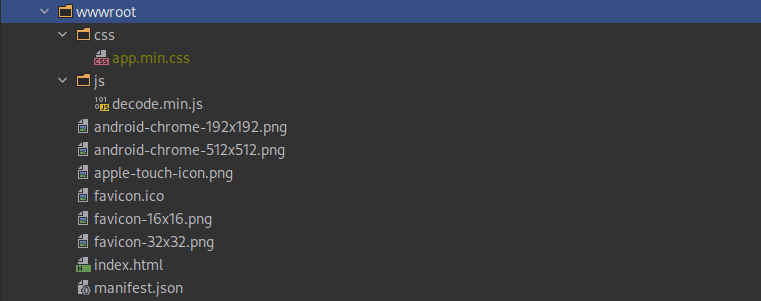
\includegraphics[width=\textwidth]{img/chapter5/wwwroot.png}
    \caption{Pliki w katalogu rdzenia webowego aplikacji klienckiej}
    \label{fig:wwwroot}
\end{figure}

Katalog wwwroot, ukazany na rys. \ref{fig:wwwroot}, znajduje się bezpośrednio w  katalogu głównym projektu aplikacji klienckiej. Nazywany jest rdzeniem webowym. Zawiera w sobie wszystkie serwowane przez system pliki statyczne.

\begin{lstlisting}[language=HTML, caption={Struktura dokumentu index.html w rdzeniu webowym aplikacji klienckiej}, label=lst:index_html]
<!DOCTYPE html>
<html class="w-full h-full">
<head>
  <meta charset="utf-8" />
  <meta content="width=device-width, initial-scale=1.0, maximum-scale=1.0, user-scalable=no" name="viewport" />
  <title>OpenOSP</title>
  <base href="/" />
  <link href="./css/app.min.css" rel="stylesheet" />
  <link href="./apple-touch-icon.png" rel="apple-touch-icon" sizes="180x180">
  <link href="./favicon-32x32.png" rel="icon" sizes="32x32" type="image/png">
  <link href="./favicon-16x16.png" rel="icon" sizes="16x16" type="image/png">
  <link href="./manifest.json" rel="manifest">
</head>
<body>
  ...
</body>
</html>
\end{lstlisting}

Dokument /wwwroot/index.html jest punktem wyjściowym aplikacji. Jego struktura, przedstawiona na listingu \ref{lst:index_html}, nie różni się niczym od struktury standardowego dokumentu, opisanego w sekcji rozdziału teoretycznego, poświęconej dokumentom HTML. W jego nagłówku, zdefiniowano metadane aplikacji, wypunktowane poniżej:

\begin{itemize}
    \item Aplikacja korzysta z systemu kodowania znaków UTF-8.
    \item Widok aplikacji wykorzystuje szerokość urządzenia, które ją wyświetla, jako szerokość strony i nie zezwala na jej skalowanie.
    \item Tytułem karty, w której otworzono aplikację, jest "OpenOSP".
    \item Dokument importuje arkusz stylów CSS z pliku /wwwroot/css/app.min.css, którego pochodzenie opisano w podsekcji poświęconej klasom Tailwind CSS.
    \item Zdefiniowane ikony są wyświetlane obok nazwy karty przeglądarki i dostępne w trzech różnych formatach. Użyte pliki graficzne są plikami statycznymi, występującymi w rdzeniu webowym aplikacji.
    \item Załączony plik manifest.json, dostarcza przeglądarkom kilka podstawowych informacji o aplikacji. Mogą okazać się one przydatne, w przypadku użycia na aplikacji mechanizmu PWA lub kontenera widoku webowego (webview container).
\end{itemize}

\begin{lstlisting}[language=HTML, caption={Treść ciała dokumentu index.html w rdzeniu webowym aplikacji klienckiej}, label=lst:index_body]
<div class="w-full h-full" id="app">
  <div class="w-full h-full flex justify-center items-center bg-base-300">
    <button class="btn btn-primary btn-outline btn-lg loading">Loading OpenOSP...</button>
  </div>
</div>
<script autostart="false" src="_framework/blazor.webassembly.js"></script>
\end{lstlisting}

Ciało dokumentu index.html, składa się z przedstawionego już wcześniej elementu o identyfikatorze "app" oraz załadowania skryptu JS, będącego częścią platformy Blazor. Początkowo, zawartość elementu app wypełniającego całe pole widoku w przeglądarce, zawiera treść informującą użytkownika o procesie ładowania aplikacji. Załączony skrypt \_framework/blazor.webassembly.js, działa w tle jako zadanie asynchroniczne, nie blokując wątku interfejsu użytkownika, wskazującego ekran ładowania. 

Skrypt pobiera potrzebne moduły WebAssembly, tworzące bardzo kompaktową implementację środowiska uruchomieniowego .NET (Mono) oraz skompilowaną do kodu pośredniego aplikację kliencką, razem z wykorzystywanymi przez nią modułami bibliotek ASP.NET Core. W praktyce, pozwala to na wykorzystanie komponentów Razor aplikacji, bezpośrednio w przeglądarce, wykorzystując webowe środowisko uruchomieniowe, jako mediator między technologiami webowymi, a technologiami .NET. 

Środowisko opiera się jedynie na standardach rekomendowanych przez W3C, dlatego nie powoduje problemów z kompatybilnością tworzonych rozwiązań. W przyszłości planuje się wprowadzenie kompilatora języka pośredniego platformy .NET, na natywny kod binarny WASM, przyspieszając proces pobierania i wykonania aplikacji w przeglądarce.

Po załadowaniu potrzebnych komponentów do pamięci przeglądarki, aplikacja Blazor uruchomiona po stronie klienta, podmienia zawartość elementu app na szablon HTML, renderowany przez komponent główny aplikacji. Został on wcześniej określony, przy pomocy odpowiedniej metody budowniczego, w metodzie Main() programu. Kolejna podsekcja opisuje, czym dokładnie są komponenty Razor i w jaki sposób wprowadzają mechanizmy aplikacji SPA po stronie klienta.

%%%%%%%%%%%%%%%%%%%%%%%%%%%%%%%%%%%%%%%%%%%%%%%%%%%%%%%%%%%%%%%%%%%%%%%%%%%%%%%%
\subsection{Komponenty Razor}
%%%%%%%%%%%%%%%%%%%%%%%%%%%%%%%%%%%%%%%%%%%%%%%%%%%%%%%%%%%%%%%%%%%%%%%%%%%%%%%%

Platforma Blazor, umożliwia tworzenie komponentów aplikacji na dwa sposoby: przy pomocy rozszerzonej notacji Razor i klas C\#. Projekt wykorzystuje pierwszą metodę, która oferuje bardziej naturalny sposób pracy z technologiami webowymi. 

W czasie budowania aplikacji, notacja zostaje przeanalizowana i przekształcona na zwykłe klasy komponentów, tak by mogło z nich skorzystać środowisko uruchomieniowe. Wykorzystanie klas bezpośrednio, jest pomocne w przypadkach zaawansowanych komponentów generycznych i funkcjonalności niedostępnych za pośrednictwem notacji Razor.

\begin{lstlisting}[language=HTML, caption={Przykładowy komponent Razor, opisujący główny układ strony}, label=lst:razor_body]
@inherits LayoutComponentBase

<div class="drawer w-auto min-h-screen text-base-content">
  <input id="navdrawer" type="checkbox" class="drawer-toggle" @bind="_isNavdrawer"/>
  <div class="drawer-content min-h-screen items-stretch">
    <div class="hero min-h-screen flex flex-col bg-firefighters">
      <div class="hero-overlay bg-opacity-70"/>
      <Header/>
      <main class="hero-content w-11/12 max-w-screen-md m-1 p-2">
        @Body
      </main>
    </div>
    <Footer/>
  </div>
  <div class="drawer-side">
    <label for="navdrawer" class="drawer-overlay"/>
    <Nav @bind-IsNavdrawer="_isNavdrawer" class="menu w-80 p-4 overflow-y-auto bg-base-300 bg-opacity-90"/>
  </div>
</div>

@code {

  private bool _isNavdrawer { get; set; }

}
\end{lstlisting}

Jako przykład komponentu, na listingu \ref{lst:razor_body} przedstawiono główny układ strony, wykorzystywany na każdej ze stron aplikacji. Rozpoczyna się od deklaracji dziedziczenia po komponencie bazowym LayoutComponentBase, przez co może zostać wykorzystany później do okalania stron w projekcie.

Kolejnym elementem jest schemat HTML, określający sposób wyświetlania komponentu na stronie. Elementy <Header>, <Footer> i <Nav> są innymi komponentami zdefiniowanymi w aplikacji, zostaną zarejestrowane w instancji aplikacji, jako obiekty swoich klas, a ich schemat zostanie wstawiony w miejsce ich znacznika. 

Znak "@" umożliwia zastosowanie języka C\# wewnątrz schematu, jeśli chcemy np. wstawić wartość pola klasy albo utworzyć blok pętli lub instrukcję warunkową. Użycie znacznika "@Body", powoduje wstawienie w jego miejsce fragmentu HTML, który został przekazany do komponentu jako zawartość, między jego znacznikiem początkowym i końcowym. 

Ostatnim elementem jest blok kodu "@code", umożliwiający łatwą definicję pól klasy komponentu, takich jak: wartości, referencje i metody. Przykładowo, zdefiniowano pole przetrzymujące wartość bool, określające czy nawigacyjny panel boczny strony jest wysunięty.

\begin{lstlisting}[language=CSharp, caption={Fragment bloku kodu komponentu Nav, poświęcony dwustronnemu wiązaniu danych}, label=lst:razor_twoWayBinding]
[Parameter]
public bool IsNavdrawer { get; set; }

[Parameter]
public EventCallback<bool> IsNavdrawerChanged { get; set; }

[Parameter(CaptureUnmatchedValues = true)]
public IReadOnlyDictionary<string, object> AdditionalAttributes { get; set; }

private async Task OnNavClick() {
  IsNavdrawer = false;
  await IsNavdrawerChanged.InvokeAsync(IsNavdrawer);
}
\end{lstlisting}

Stan komponentów nie jest składowany przy pomocy dedykowanego mechanizmu stanu, a jedynie wewnątrz ich obiektów (pamięć WASM). Dlatego, ważnym mechanizmem w aplikacji są dowiązania danych. Na listingu \ref{lst:razor_body}, komponent układu strony dzieli się z komponentem Nav, wartością pola \_isNavdrawer przy pomocy atrybutu "@bind-Navdrawer".

Jest to specjalny rodzaj notacji umożliwiający dowiązanie dwukierunkowe, w którym obiekt emitujący wartość pola, może zostać powiadomiony o zmianie tej wartości, za pośrednictwem mechanizmu zdarzeń (Event).

W rzeczywistości,  atrybut na listingu \ref{lst:razor_twoWayBinding}, przypisuje wartość dwóm parametrom komponentu Nav. Pierwszy to IsNavdrawer przetrzymujący wartość przekazanego pola, a drugi to IsNavdrawerChanged definiujący zdarzenie wywoływane, aby zaktualizować wartość przekazywanego pola w komponencie emitującym.

Przykładowo, przy kliknięciu na link w panelu bocznym, jest on chowany przy pomocy metody OnNavClick(). Najpierw podmieniana jest wartość IsNavdrawer, a następnie wywołuje się zdarzenie, przekazujące nową wartość komponentowi nadrzędnemu, będącego tzw. konsumentem zdarzenia.

Parametry komponentów, są publicznymi polami klasy, zdefiniowanymi w bloku kodu komponentu i oznaczone adnotacją Parameter. W prostszym przypadku mogą służyć przekazaniu wartości jednostronnie, pomijając prefiks "@bind-" atrybutu, w schemacie komponentu emitującego. Aby wykorzystać atrybuty nie przekazane do konkretnego pola parametru, należy zdefiniować pole kolekcji par klucz-wartość i oznaczyć je adnotacją Parameter, wraz z opcjonalnym argumentem flagi CaptureUnmatchedValues.

\begin{lstlisting}[language=CSharp, caption={Fragmenty komponentu tabeli członków zespołu wykorzystujące kaskadowe parametry}, label=lst:razor_cascadingParameters]
...
    <tbody>
    @foreach (var member in _members) {
      <CascadingValue Value=@member>
        <MemberRecord OnUpdateCallback="UpdateTable"/>
      </CascadingValue>
    }
    </tbody>
...

@code {

  [CascadingParameter(Name = "CheckedMembers")]
  private IDictionary<int, string> _checkedMembers { get; set; }

  private IEnumerable<MemberReadDto> _members { get; set; } = new List<MemberReadDto>();
  ...
}
\end{lstlisting}

\begin{lstlisting}[language=CSharp, caption={Kaskadowe parametry, komponentu rekordu tabeli członków zespołu}, label=lst:razor_memberRecord]
[CascadingParameter]
private MemberReadDto _readDto { get; set; }

[CascadingParameter(Name = "CheckedMembers")]
private IDictionary<int, string> _checkedMembers { get; set; }
\end{lstlisting}

Zwykłe atrybuty, nie są jedynym sposobem na jednostronne przekazanie wartości między komponentami. Za pomocą tzw. kaskadowych parametrów, można znacznie uprościć sytuacje przekazywania tej samej wartości przez wiele warstw komponentów. 

Jest to możliwe, dzięki znacznikowi <CascadingValue>, przyjmującego atrybut Value, określający wartość do przekazania w dół hierarchii komponentów. Opcjonalny atrybut Name, ustanawia identyfikator emitowanej wartości, pozwalając na rozwiązanie konfliktów między kaskadowymi parametrami tego samego typu.

Przykład wykorzystania kaskadowych parametrów został pokazany na listingu \ref{lst:razor_cascadingParameters}. Do obiektów komponentu rekordu tabeli, utworzonych w pętli foreach, kaskadowo przekazuje się obiekty reprezentacji odczytu członków zespołu, pozyskanych z bazy danych. Każdy rekord odbiera go przy pomocy pola \_readDto, oznaczonego przez adnotacje CascadingParameter, ukazanego na listingu \ref{lst:razor_memberRecord}.

W odróżnieniu od zwykłych parametrów, parametry kaskadowe mogą korzystać z pól niepublicznych. Parametry przekazywane między komponentami Razor, podlegają rozróżnieniu na typy referencyjne i przekazywane przez wartość. Domyślnie, wartości te wpisywane są do oznaczonych pól posiadających ten sam typ, co emitowana wartość. 

Komponenty tabeli i rekordu zawierają pole kaskadowego parametru, przekazywanego przez identyfikator "CheckedMembers". Pierwszy z nich wykorzystuje go w przypadku usuwania zaznaczonych wartości, drugi indykuje stan zaznaczenia w swoim schemacie, bazując na zawartości kolekcji.

\begin{lstlisting}[language=CSharp, caption={Fragmenty komponentu logowania użytkownika, wykorzystujące zastrzyki zależności i bloki warunkowe}, label=lst:razor_dependencyInjection]
@inject IAuthenticationService _authService
@inject NavigationManager _navManager

...
    <button type="submit" class="@($"btn btn-primary {(isWaitingForResult ? "loading" : string.Empty)}")" disabled="@isWaitingForResult">
      @if (isWaitingForResult is false) {
        <span>Log in</span>
      }
      else {
        <span>Logging in...</span>
      }
    </button>
...

@code {

  private UserLoginDto _dto = new();

  private bool isWaitingForResult = false;
  
  ...

  private async Task HandleLogin() {
    isWaitingForResult = true;
    showAuthenticationError = false;
    var result = await _authService.Login(_dto);
    if (result is not null) {
      _navManager.NavigateTo("/userpanel");
    }
    else {
      isWaitingForResult = false;
      authenticationError = "There was a problem logging in";
      showAuthenticationError = true;
    }
  }
}
\end{lstlisting}

Komponenty Razor mogą korzystać z zastrzyków zależności, deklarując zależność od wybranych serwisów przy pomocy znacznika "@inject". Wstrzyknięte w ten sposób serwisy są dostępne w całym bloku kodu komponentu, jak i jego schemacie, pod nazwą wskazaną w deklaracji zależności. W rzeczywistości, wstrzykiwanie zostaje przeprowadzone w konstruktorze wygenerowanej klasy komponentu.

Jednym z zarejestrowanych domyślnie serwisów, jest NavigationManager, wstrzykiwany przykładowo na listingu \ref{lst:razor_dependencyInjection}. Jego metody stanowią alternatywny, do nawigacyjnych linków HTML, sposób nawigacji po stronach aplikacji. Najczęściej są wykorzystywane do automatyzacji tego procesu, w metodach komponentów.

Listing zawiera przykłady wykorzystania bloków warunkowych w notacji Razor. Wyrażenia warunkowe można stosować nie tylko pomiędzy kolejnymi znacznikami HTML, ale również w ich atrybutach. Pozwala to na skrócenie schematu komponentu i uniknięcie powtórzeń.

Atrybut disabled zastosowany w elemencie przycisku, stanowi przykład rozbudowania funkcjonalności standardu HTML. W zwykłym dokumencie jest on wykorzystywany jako flaga, wskazująca na nieaktywność elementu w interfejsie użytkownika, bez względu na przypisaną mu wartość. Notacja Razor umożliwia dowiązania do niego wartości bool, z pomocą której można dynamicznie włączać i wyłączać tą flagę.

\begin{lstlisting}[language=CSharp, caption={Komponent Razor tworzący odnośniki do swojej zawartości, przy pomocy znaczników page}, label=lst:razor_home]
@page "/"
@page "/about"
@page "/contact"
@page "/verify/{verificationString}"

...

@code {

  [Parameter]
  public string VerificationString { get; set; }

  private bool showVerificationSuccess = false;

  protected override async Task OnInitializedAsync() {
    if (string.IsNullOrEmpty(VerificationString) is false) {
      var verificationResult = await _http.GetAsync($"api/users/verify?{VerificationString}");
      if (verificationResult.IsSuccessStatusCode) {
        showVerificationSuccess = true;
      }
    }
  }

  protected override async Task OnAfterRenderAsync(bool firstRender) {
    if (firstRender && showVerificationSuccess) {
      await Task.Delay(10000);
      showVerificationSuccess = false;
      StateHasChanged();
      NavManager.NavigateTo("/");
    }
  }

}
\end{lstlisting}

Niektóre komponenty, przy pomocy znacznika @page, deklarują ścieżki URI punktów końcowych, dla których ich schemat zostanie wyrenderowany na stronie aplikacji. Można zadeklarować więcej niż jedną, prowadzącą do treści ścieżkę. Podobnie jak w przypadku punktów końcowych aplikacji serwerowej, ścieżki mogą zawierać w sobie wartości parametrów, które zostaną przypisane do pól oznaczonych jako parametry w kodzie komponentu.

Strona główna aplikacji, przedstawiona na listingu \ref{lst:razor_home}, pełni jednocześnie funkcję strony weryfikującej e-mail zarejestrowanego użytkownika. Pobierając wartość łańcucha weryfikacyjnego, przesyła jego treść w zapytaniu żądania do kontrolera aplikacji serwerowej, wykorzystując metodę OnInitializedAsync() wywoływaną po inicjalizacji komponentu. Druga z metod OnAfterRenderAsync(), wywoływana jest po zakończeniu renderowania komponentu. Po upływie 10 sekund od pierwszego wyrenderowania komponentu na stronie, likwiduje informację o udanej weryfikacji e-maila i przekierowuje użytkownika do ścieżki "/".

Obie funkcje stanowią przykład metod wirtualnych, dziedziczonych po implikowanej klasie bazowej, wywoływanych automatycznie w danym momencie cyklu życia komponentu Razor. Nadpisując ciała tych metod, można określić dokładny moment wykonania wybranych procedur związanych z danym komponentem lub jego pochodnymi.

\begin{lstlisting}[language=CSharp, caption={Główny komponent Razor aplikacji klienckiej}, label=lst:razor_app]
@using OpenOsp.Client.Components.Main
<Router AppAssembly="@typeof(Program).Assembly" PreferExactMatches="true">
  <Found Context="routeData">
    <AuthorizeRouteView RouteData="@routeData" DefaultLayout="@typeof(Body)">
      ...
    </AuthorizeRouteView>
  </Found>
  <NotFound>
    <CascadingAuthenticationState>
      <LayoutView Layout="typeof(Body)">
        <OpenOsp.Client.Pages.NotFound/>
      </LayoutView>
    </CascadingAuthenticationState>
  </NotFound>
</Router
\end{lstlisting}

Schemat głównego komponentu aplikacji, widoczny na listingu \ref{lst:razor_app}, odpowiada za wewnętrzne trasowanie do komponentów-stron. Element Router wykorzystuje informacje o bibliotece klas aplikacji klienckiej, w celu sporządzenia listy ścieżek punktów końcowych, dla których wyrenderowana zostanie odpowiednia zawartość. 

Element Found obsługuje sytuację odnalezienia komponentu-strony, pod wskazaną ścieżką, wstawiając jego schemat w środku głównego układu strony, pokazanego na listingu \ref{lst:razor_body}. W przypadku nie odnalezienia komponentu-strony pod wskazaną ścieżką, wyświetlony zostanie dedykowany tej sytuacji komponent, określony w elemencie NotFound.

\begin{figure}[!htbp] 
    \centering
    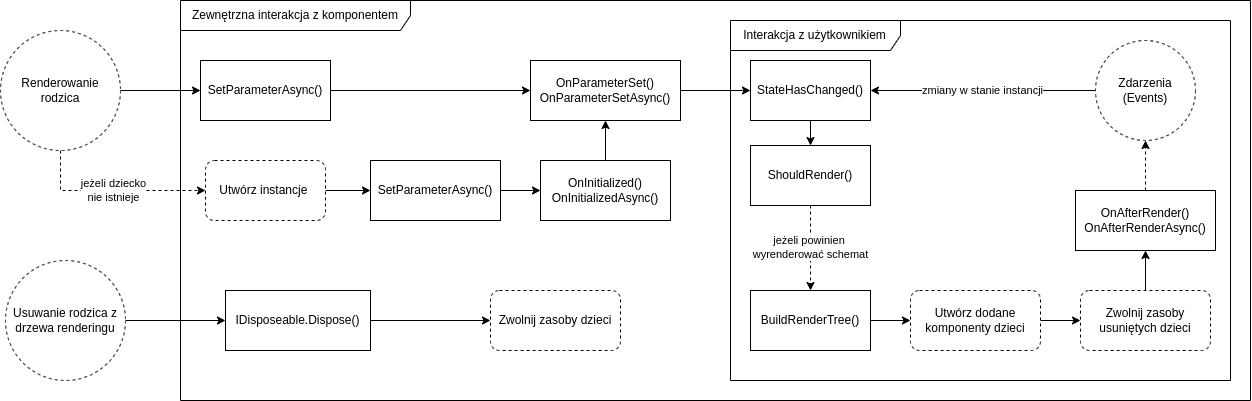
\includegraphics[width=\textwidth]{img/chapter5/razor.lifecycle.png}
    \caption{Cykl życia komponentów Razor}
    \label{fig:razor.lifecycle}
\end{figure}

Na rys. \ref{fig:razor.lifecycle} zaprezentowano cykl życia komponentów Razor. Struktura renderowanych przez aplikacje komponentów jest drzewem ich instancji, w którym korzeń stanowi unikatowa instancja komponentu App. Wewnątrz tego grafu, zmiany dokonane na instancji komponentu nadrzędnego (rodzica), implikują przymus ponownego wyrenderowania go i wszystkich podrzędnych mu instancji (dzieci). Jest to mechanizm optymalizacyjny aplikacji graficznych, tworzący podstawę działania aplikacji SPA. 

%%%%%%%%%%%%%%%%%%%%%%%%%%%%%%%%%%%%%%%%%%%%%%%%%%%%%%%%%%%%%%%%%%%%%%%%%%%%%%%%
\subsection{Generowanie arkusza CSS}
%%%%%%%%%%%%%%%%%%%%%%%%%%%%%%%%%%%%%%%%%%%%%%%%%%%%%%%%%%%%%%%%%%%%%%%%%%%%%%%%

W projekcie aplikacji zostały użyte narzędzia platformy NodeJS. W celu uproszczenia procesu stylizacji komponentów, zastosowano oparte o technologię JavaScript pakiety: TailwindCSS, Autoprefixer, CSSNano i PostCSS. 

\begin{lstlisting}[language=JavaScript, caption={Plik package.json w aplikacji klienckiej}, label=lst:package.json]
{
  ...
  "scripts": {
    "buildcss:dev": "cross-env TAILWIND_MODE=build postcss ./Styles/app.css -o ./wwwroot/css/app.min.css",
    "buildcss": "postcss ./Styles/app.css -o ./wwwroot/css/app.min.css"
  },
  ...
  "devDependencies": {
    "autoprefixer": "^10.3.4",
    "cross-env": "^7.0.3",
    "cssnano": "^5.0.8",
    "daisyui": "^1.14.0",
    "postcss": "^8.3.6",
    "postcss-cli": "^8.3.1",
    "tailwindcss": "^2.2.9",
    "tailwindcss-textshadow": "^2.1.3"
  }
}
\end{lstlisting}

Fragment pliku package.json, przedstawiony na listingu \ref{lst:package.json}, definiuje zbiór pakietów NodeJS potrzebnych podczas budowania aplikacji oraz dodatkowe skrypty pomocnicze. Narzędzie PostCSS, za pośrednictwem swoich rozszerzeń, wykorzystuje mechanizmy pozostałych trzech pakietów na wskazanym pliku wejściowym /Style/app.css. Umieszczony w rdzeniu webowym arkusz app.min.css, załączony w nagłówku dokumentu index.html, jest plikiem wynikowym tej operacji.

\begin{lstlisting}[language=CSS, caption={Plik /Styles/app.css w aplikacji klienckiej}, label=lst:app.css]
@tailwind base;
@tailwind components;
@tailwind utilities;
\end{lstlisting}

Plik /Styles/app.css zawiera kwerendy platformy TailwindCSS, wykorzystywane w procesie generacji arkusza CSS, używanego przez aplikację. W ich miejsce wstawiane są klasy CSS odpowiednich rodzajów, zdefiniowane przez pakiet.

\begin{lstlisting}[language=CSS, caption={Konfiguracja narzędzia TailwindCSS w pliku tailwind.config.js}, label=lst:tailwind]
module.exports = {
  mode: 'jit',
  purge: [
    './wwwroot/index.html',
    './**/*.razor',
  ],
  ...
}
\end{lstlisting}

Aby uniknąć generacji klas CSS niewykorzystywanych w projekcie, można zastosować tzw. generację w locie wraz z trybem czystki. Na listingu \ref{lst:tailwind}, deklarowane jest, że narzędzie powinno umieścić w pliku app.min.css tylko te klasy TaliwindCSS, które zostały wykorzystane przez dokument index.html lub którykolwiek z komponentów Razor, na wszystkich poziomach zagnieżdżenia projektu.

\begin{lstlisting}[language=HTML, caption={Fragment pliku OpenOsp.Client.csproj, automatyzujący generację arkusza CSS projektu}, label=lst:client_csproj]
<Target Name="NpmCheck" BeforeTargets="NpmInstall">
  <Exec Command="npm -v" ContinueOnError="true">
    <Output TaskParameter="ExitCode" PropertyName="ErrorCode" />
  </Exec>
  <Error Condition="'$(ErrorCode)' != '0'" Text="NPM not found. Please install Node.js and npm first." />
</Target>
<Target Name="NpmInstall" BeforeTargets="BuildCss" Inputs="./package.json" Outputs="$(NpmLastInstall)">
  <Exec Command="npm ci" />
  <Touch Files="$(NpmLastInstall)" AlwaysCreate="true" />
</Target>
<Target Name="BuildCss" BeforeTargets="Compile">
  <Exec Command="npm run buildcss" />
</Target>
\end{lstlisting}

Proces generacji klas i minimalizacji otrzymanego arkusza CSS, został zautomatyzowany przy pomocy konfiguracji w pliku OpenOsp.Client.csproj widocznej na listingu \ref{lst:client_csproj}. Notacja MSBuild sprawdza dostępność konsolowego menadżera pakietów npm i w razie potrzeby, instaluje nieobecne pliki pakietów NodeJS. Na końcu uruchamiany jest skrypt npm, zdefiniowany wcześniej w pliku package.json, generujący arkusz stylów aplikacji w rdzeniu webowym, jeszcze przed rozpoczęciem procesu kompilacji projektu.

%%%%%%%%%%%%%%%%%%%%%%%%%%%%%%%%%%%%%%%%%%%%%%%%%%%%%%%%%%%%%%%%%%%%%%%%%%%%%%%%
\subsection{Formularze i walidacja danych}
%%%%%%%%%%%%%%%%%%%%%%%%%%%%%%%%%%%%%%%%%%%%%%%%%%%%%%%%%%%%%%%%%%%%%%%%%%%%%%%%

Formularze danych to jedne z ważniejszych elementów interfejsu użytkownika. Twórcy platformy Blazor, zdefiniowali zbiór komponentów ułatwiających dowiązywanie danych, w polach formularza i wyświetlanie informacji zwrotnej o przebiegu ich walidacji.

\begin{lstlisting}[language=CSharp, caption={Przykład formularza danych w aplikacji klienckiej}, label=lst:editForm]
@inject HttpClient _http

...
  <EditForm Model="@_createDto" OnValidSubmit="HandleCreate" class="modal-box">
    ...
    <h1 class="mb-5 text-center text-2xl font-bold">Create a member</h1>
    <DataAnnotationsValidator/>
    <LabeledInputText @bind-Value="_createDto.FirstName"/>
    <LabeledInputText @bind-Value="_createDto.LastName"/>
    <LabeledInputText @bind-Value="_createDto.Pesel"/>
    <div class="modal-action">
      <button type="submit" class="@($"btn btn-primary {(isWaitingForResponse ? "loading" : string.Empty)}")" hidden="@isWaitingForResponse">Create</button>
      <label for="member-create-modal" class="btn" hidden="@isWaitingForResponse">Cancel</label>
    </div>
  </EditForm>
...

@code {
  
  ...
  private MemberCreateDto _createDto { get; set; } = new();
  ...

  private async Task HandleCreate() {
    showError = false;
    isWaitingForResponse = true;
    var result = await _http.PostAsJsonAsync("api/members", _createDto);
    isWaitingForResponse = false;
    ...
  }
  ...
}
\end{lstlisting}

Komponent EditForm jest wykorzystywany, do okalania formularzy, zamiast standardowego elementu <form>. Posiada osobne atrybuty, pozwalające określić metody obsługujące próby przesłania formularza dla danych poprawnych OnValidSubmit oraz dla niepoprawnych OnInvalidSubmit. Do przesyłania danych w formularzu, służy zwykły przycisk HTML typu submit.

Model danych, który podlega walidacji przez komponent formularza, jest przekazywany w atrybucie Model. Aby skorzystać z rezultatów walidacji poszczególnych pól formularza, przy pomocy ich adnotacji, należy umieścić dodatkowy komponent walidatora DataAnnotationsValidator, w zawartości formularza. 

\begin{lstlisting}[language=CSharp, caption={Rozszerzony komponent pola tekstowego formularza w aplikacji klienckiej}, label=lst:inputText]
@inherits InputText

<div class="form-control">
  @if (IsLabeled) {
    <label class="label">
      <LabelText For="@ValueExpression" class="label-text"/>
    </label>
  }
  <InputText @attributes="AdditionalAttributes"
             Value="@Value" ValueChanged="@ValueChanged" ValueExpression="@ValueExpression"
             class=@("input input-bordered " + CssClass.Replace(" valid", " input-success").Replace(" invalid", " input-error"))/>
  <label class="label">
    @SubLabel
    <div class="label-text-alt mx-2 text-error text-xs">
      <ValidationMessage For="@ValueExpression"/>
    </div>
  </label>
</div>
\end{lstlisting}

Komponent pola tekstowego, definiowanego przez platformę Razor, został rozszerzony w sposób pokazany na listingu \ref{lst:inputText}. Korzystając z biblioteki rozszerzeń formularzy, nad polem zostaje wyświetlona jego wizualna nazwa. Nazwy określić można w adnotacji Display, którą oznacza się pole klasy obiektu transferu danych (patrz listing \ref{lst:member_update_dto}).

% obraz udanej walidacji
\begin{figure}[!htbp]
\centering
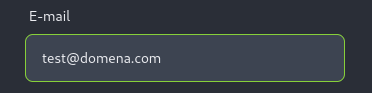
\includegraphics[width=\textwidth]{img/chapter5/form_valid.png}
\caption{Przykład udanej walidacji pola formularza}
\end{figure}

% obraz nieudanej walidacji
\begin{figure}[!htbp]
\centering
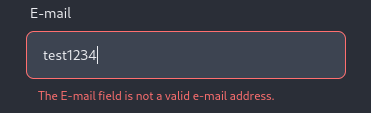
\includegraphics[width=\textwidth]{img/chapter5/form_invalid.png}
\caption{Przykład nieudanej walidacji pola formularza}
\end{figure}

Rezultat walidacji indykowany jest przy pomocy koloru obramowania pola tekstowego, ustawianego w dodatkowej logice stosowanej na klasach elementu. W przypadku niepowodzenia, wyświetlany jest komunikat o błędach walidacji.

%%%%%%%%%%%%%%%%%%%%%%%%%%%%%%%%%%%%%%%%%%%%%%%%%%%%%%%%%%%%%%%%%%%%%%%%%%%%%%%%
\section{Użytkownicy systemu}
%%%%%%%%%%%%%%%%%%%%%%%%%%%%%%%%%%%%%%%%%%%%%%%%%%%%%%%%%%%%%%%%%%%%%%%%%%%%%%%%

Interakcja z użytkownikami systemu, oparta jest o klasy biblioteki tożsamości ASP.NET Core, odpowiedzialnych m.in. za mechanizmy uwierzytelniania i autoryzacji w systemie. Aby składować informacje o użytkownikach i ich stanie, w bazie danych aplikacji, zaimportowano dedykowane temu rozszerzenie EF Core.

\begin{lstlisting}[language=CSharp, caption={Klasa zasobu użytkownika systemu}, label=lst:user]
public class User : IdentityUser<int> {
  ...
}
\end{lstlisting}

Na listingu \ref{lst:user}, klasa zasobu użytkownika rozszerza klasę generyczną IdentityUser, określając typ klucza głównego (identyfikatora) jako liczbę całkowitą. Dziedziczenie jest jednoznaczne z implementacją interfejsu, łączącego logicznie encje użytkowników i moduły biblioteki tożsamości.

\begin{lstlisting}[language=CSharp, caption={Konfiguracja serwisów związanych z użytkownikami w metodzie Startup.ConfigureServices()}, label=lst:config_users]
services.Configure<JwtSettings>(Configuration.GetSection("Jwt"));
services.Configure<EmailSettings>(Configuration.GetSection("Email"));
...
services.AddIdentityCore<OspM.User>(cfg => {
    cfg.User.RequireUniqueEmail = true;
    cfg.Password.RequireDigit = false;
    cfg.Password.RequireLowercase = false;
    cfg.Password.RequireUppercase = false;
    cfg.Password.RequireNonAlphanumeric = false;
    cfg.Password.RequiredLength = 12;
    cfg.SignIn.RequireConfirmedEmail = true;
  })
  .AddEntityFrameworkStores<AppDbContext>()
  .AddDefaultTokenProviders()
  .AddUserManager<UserManager<OspM.User>>()
  .AddSignInManager<SignInManager<OspM.User>>();
...
services.AddScoped<IEmailsService, EmailsService>();
services.AddScoped<IUserService<OspM.User, int>, UserService<OspM.User, int>>();
services.AddScoped<IUserClaimsService<int>, UserClaimsService<int>>();
\end{lstlisting}

Listing \ref{lst:config_users}, rozpoczyna się od rejestracji konfiguracyjnych struktur danych, związanych z wiadomościami e-mail oraz tokenami JWT. Struktury są wstrzykiwane do zależnych od nich klientów, podobnie jak w przypadku serwisów warstwy logiki.

W drugiej kolejności, skonfigurowane zostają serwisy tożsamości. Metoda budowniczego, dodana przez bibliotekę tożsamości, rejestruje wykorzystanie klasy zasobu użytkownika zdefiniowanej na listingu \ref{lst:user}, za pomocą parametru typu. Wyrażenie lambda w argumentach, przekazuje do metody, klasę konfiguracyjną serwisów tożsamości. Na użytkowników nakładany jest przymus rejestracji, przy pomocy unikatowego adresu e-mail oraz potwierdzenia go przed próbą uwierzytelnienia. Natomiast, łańcuchy haseł muszą zawierać przynajmniej 12 dowolnych znaków.

Dalsze biegłe wywołania, rejestrują serwis odpowiedzialny za przetrzymywanie danych, związanych z tożsamością w bazie danych i tzw. menadżerów użytkowników oraz uwierzytelniania. Menadżerowie stanowią mediator, między tabelami modułów tożsamości, a zależnymi od nich klientami zdefiniowanymi przez programistę. Ich obowiązki, można porównać do klas repozytoriów, jednakże wprowadzają o wiele grubszą warstwę abstrakcji, związaną z operacjami takimi jak: haszowanie haseł, weryfikowanie adresów e-mail lub próba uwierzytelnienia użytkownika.

\begin{lstlisting}[language=CSharp, caption={Konfiguracja tokenów JWT jako mechanizmu niosącego w sobie dane uwierzytelniające}, label=lst:config_jwt]
services.AddAuthentication()
  .AddJwtBearer(cfg => {
    cfg.TokenValidationParameters = new TokenValidationParameters {
      ValidIssuer = Configuration["Jwt:Issuer"],
      ValidateIssuer = true,
      ValidAudience = Configuration["Jwt:Audience"],
      ValidateAudience = true,
      IssuerSigningKey = new SymmetricSecurityKey(Encoding.UTF8.GetBytes(Configuration["Jwt:Key"])),
      RequireSignedTokens = true,
      RequireExpirationTime = true,
      ValidateLifetime = true
    };
  });
\end{lstlisting}

\begin{lstlisting}[language=CSharp, caption={Konfiguracja tokenów JWT w pliku appsettings.json}, label=lst:appsettings_jwt]
"Jwt": {
  "Key": "<3AH17ZH<zg[aHp0&BJV5?b0;*TA$/&p",
  "Issuer": "https://api.openosp.com/",
  "Audience": "users"
},
...
\end{lstlisting}

Konfiguracja mechanizmu uwierzytelniającego, na listingu \ref{lst:config_jwt}, dodaje obsługę schematu autoryzacji przy pomocy tokenów JWT, niosących w sobie dane uwierzytelniające. Przy pomocy sekcji ustawień z pliku appsettings.json, pokazanej na listingu \ref{lst:appsettings_jwt}, wyrażenie lambda konfiguruje wymóg podania informacji o emitencie oraz odbiorcach tokena i sekretny klucz wykorzystywany przez podpisujący je algorytm. Wymagane jest również podawanie terminu ważności tworzonych tokenów na etapie ich tworzenia.

Wszystkie z tych informacji, zostają sprawdzone podczas autoryzacji dostępu do klas lub pól oznaczonych adnotacją Authorize, które deklarują wykorzystanie zarejestrowanego schematu, tak jak robi to kontroler autoryzowany z listingu \ref{lst:authorizedController}. W wyniku, automatycznie odmawia się dostępu nieuwierzytelnionym klientom, do wybranych lub wszystkich punktów końcowych kontrolera. Chcąc wyłączyć autoryzację dla konkretnego pola klasy, można oznaczyć je przy pomocy adnotacji NotAuthorized.

%%%%%%%%%%%%%%%%%%%%%%%%%%%%%%%%%%%%%%%%%%%%%%%%%%%%%%%%%%%%%%%%%%%%%%%%%%%%%%%%
\subsection{Tworzenie nowych użytkowników}
%%%%%%%%%%%%%%%%%%%%%%%%%%%%%%%%%%%%%%%%%%%%%%%%%%%%%%%%%%%%%%%%%%%%%%%%%%%%%%%%

% obraz formularza rejestracji
\begin{figure}[!htbp]
\centering

\includegraphics[width=\textwidth]{img/chapter5/registration.png}
\caption{Wypełniony formularz rejestracji, oczekujący na odpowiedź serwera}
\end{figure}

Proces rejestracji nowego użytkownika w systemie, rozpoczyna się od uzupełnienia jego danych w formularzu rejestracji i potwierdzenia ich przesłania. Formularz Razor wywołuje asynchroniczną metodę, przesyłającą żądanie "POST /api/users/register" do aplikacji serwerowej.

\begin{lstlisting}[language=CSharp, caption={Metoda kontrolera użytkowników odpowiedzialna za rejestrację nowego użytkownika w systemie}, label=lst:users_register]
[HttpPost("register")]
public async Task<ActionResult> Register([FromBody] UserRegisterDto dto) {
  try {
    if (TryValidateModel(dto) == false) {
      throw new ValidationProblemException();
    }
    var user = _mapper.MapRegister(dto);
    await _service.Create(user, dto.Password);
    var token = await _service.GetEmailConfirmationToken(user);
    var link = $"https://localhost:5001/verify/uid={user.Id}&token={token}";
    await _emailsService.SendVerificationEmail(user.Email, link);
    return Ok();
  }
  ...
}
\end{lstlisting}

Żądanie jest obsługiwane przez kontroler użytkowników, w metodzie Register() widocznej na listingu \ref{lst:users_register}. Za pomocą adnotacji FromBody, możliwe jest użycie ciała żądania jako argumentu metody. Po udanej walidacji danych formularza, jest on mapowany na nowy obiekt użytkownika i przekazywany wraz z łańcuchem hasła do metody serwisu, dedykowanej tworzeniu nowych użytkowników.

W przypadku powodzenia operacji, obiekt nowego użytkownika staje się mapowaną przez ORM reprezentacją encji. Z jego pomocą, generowany jest token potwierdzający adres e-mail, przesyłany następnie, na wskazany w procesie rejestracji adres, za pośrednictwem wstrzykniętego serwisu.

\begin{lstlisting}[language=CSharp, caption={Fragment serwisu mailowego aplikacji serwerowej}, label=lst:emailService]
public class EmailsService : IEmailsService {
  private readonly EmailSettings _emailSettings;

  public EmailsService(IOptions<EmailSettings> emailSettings) {
    _emailSettings = emailSettings.Value;
  }

  public async Task SendVerificationEmail(string email, string link) {
    var body = $@"
        ...
        <p>Please click <a href=""{link}"" target=""_blank"">this link</a> to confirm your email :)</p>
        ";
    await SendEmail(email, "OpenOSP Email Verification", body);
  }

  public async Task SendEmail(string email, string subject, string body) {
    using (var client = new SmtpClient()) {
      client.Host = _emailSettings.Server;
      ...
      await client.SendMailAsync(new MailMessage(_emailSettings.Address, email) {
        From = new MailAddress(_emailSettings.Address, _emailSettings.Name),
        Subject = subject,
        Body = body,
        IsBodyHtml = true,
        BodyEncoding = Encoding.UTF8
      });
    }
  }
}
\end{lstlisting}

Serwis e-mailowy aplikacji, pokazany na listingu \ref{lst:emailService}, korzysta z konfiguracji przekazanej z pliku appsettings.json, za pośrednictwem wstrzykniętej struktury EmailSettings. Obiekt klienta SMTP, stanowi przykład klasy wykorzystującej tzw. pamięć niezarządzalną, której zwalnianie przebiega za pośrednictwem interfejsu IDisposeable.

W bloku using, ograniczającym czas życia obiektu, tworzona jest konfiguracja klienta SMTP, umożliwiająca przesłanie wiadomości e-mail zawierającej w sobie link aktywacyjny. Celem zastosowania bloków i wyrażeń using, jest automatyczne wywoływanie metody Dispose(). W tym przypadku, służy ona poprawnemu zamknięciu połączenia z serwerem SMTP (przykład pamięci niezarządzalnej), po ukończeniu procedur wewnątrz bloku lub w sytuacji rzucenia wyjątku w jego wnętrzu.

% obraz otrzymanego maila
\begin{figure}[!htbp]
\centering
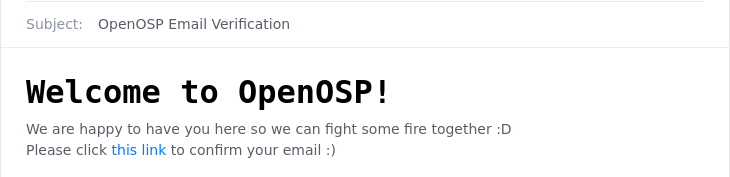
\includegraphics[width=\textwidth]{img/chapter5/email_content.png}
\caption{Wiadomość e-mail z linkiem potwierdzającym adres użytkownika}
\end{figure}

\begin{lstlisting}[language=CSharp, caption={Metoda kontrolera użytkowników, weryfikująca adres e-mail użytkownika}, label=lst:users_verify]
[HttpGet("verify")]
public async Task<ActionResult> Verify([FromQuery] int uid, [FromQuery] string token) {
  try {
    var user = await _service.ReadById(uid);
    await _service.ConfirmEmail(user, token);
    return Ok();
  }
  ...
}
\end{lstlisting}
 
Po przejściu na stronę wskazaną przez link aktywacyjny, komponent strony głównej, z listingu \ref{lst:razor_home}, wykorzystuje parametr przekazany przez URI, wysyłając żądanie obsługiwane przez metodę Verify() ukazaną na listingu \ref{lst:users_verify}. Identyfikator użytkownika oraz token potwierdzający, są przekazywane do argumentów metody, przy pomocy adnotacji FromQuery, odpowiedzialnej za obsługę tzw. zapytań URI.

% obraz strony głównej po kliknięciu w link aktywacyjny (lub sama belka potwierdzenia)
\begin{figure}[!htbp]
\centering

\includegraphics[width=\textwidth]{img/chapter5/confirmed.png}
\caption{Komunikat potwierdzenia adresu e-mail użytkownika}
\label{fig:confirmation}
\end{figure}

W przypadku udanej próby potwierdzenia adresu, na stronie głównej zostaje wyświetlony komunikat, widoczny na rys. \ref{fig:confirmation}. Komunikat znika po upływie 10 sekund, tak jak zostało to opisane pod listingiem \ref{lst:razor_home}.

%%%%%%%%%%%%%%%%%%%%%%%%%%%%%%%%%%%%%%%%%%%%%%%%%%%%%%%%%%%%%%%%%%%%%%%%%%%%%%%%
\subsection{Uwierzytelnianie i usuwanie danych uwierzytelniających}
%%%%%%%%%%%%%%%%%%%%%%%%%%%%%%%%%%%%%%%%%%%%%%%%%%%%%%%%%%%%%%%%%%%%%%%%%%%%%%%%

% obraz formularza logowania
\begin{figure}[!htbp]
\centering
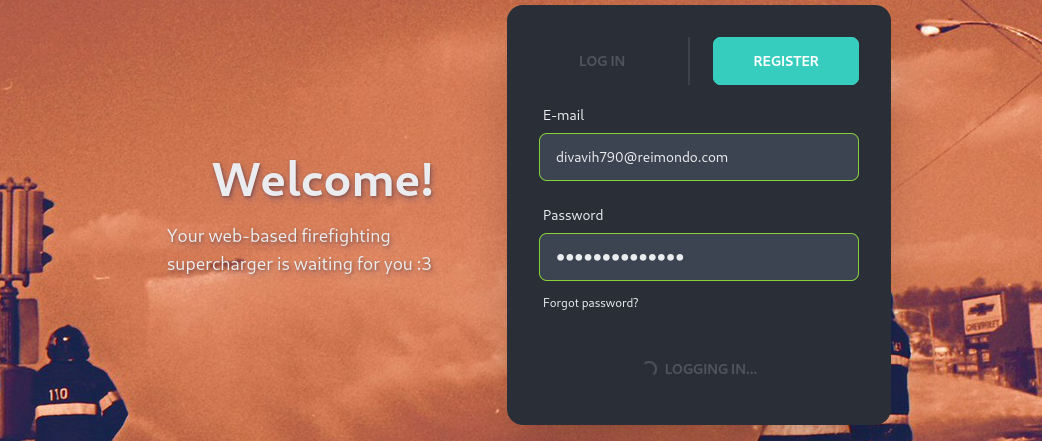
\includegraphics[width=\textwidth]{img/chapter5/login.png}
\caption{Wypełniony formularz logowania oczekujący na odpowiedź serwera}
\label{fig:form_login}
\end{figure}

Uwierzytelnianie użytkownika odbywa się poprzez formularz logowania widoczny na rys. \ref{fig:form_login}. Metoda obsługująca zdarzenie przesłania danych formularza, korzysta ze wstrzykniętego serwisu uwierzytelniania.

\begin{lstlisting}[language=CSharp, caption={Metoda uwierzytelniająca użytkownika, w klasie serwisu uwierzytelniającego aplikacji klienckiej}, label=lst:login_request]
public async Task<string> Login(UserLoginDto loginDto) {
  var authResult = await _http.PostAsJsonAsync("api/users/login", loginDto);
  var authContent = await authResult.Content.ReadAsStringAsync();
  if (authResult.IsSuccessStatusCode is false) {
    return null;
  }
  ...
}
\end{lstlisting}

\begin{lstlisting}[language=CSharp, caption={Metoda kontrolera użytkowników, obsługująca żądanie uwierzytelniające}, label=lst:users_login]
[HttpPost("login")]
public async Task<ActionResult<string>> Login([FromBody] UserLoginDto dto) {
  try {
    if (TryValidateModel(dto) == false) {
      throw new ValidationProblemException();
    }
    var user = await _service.ReadByEmail(dto.Email);
    var token = await _service.GetAuthenticationToken(user, dto.Password);
    return Ok(token);
  }
  ...
}
\end{lstlisting}

Ciało metody Login(), przedstawionej na listingu \ref{lst:login_request}, rozpoczyna się od przesłania żądania "POST /api/users/login", z danymi logowania w formacie JSON, przekazanym przez komponent. Żądanie, obsługiwane jest przez metodę kontrolera użytkowników, widoczną na listingu \ref{lst:users_login}. Przy pomocy encji użytkownika wyszukanej po adresie e-mail, wywoływana jest metoda serwisu użytkowników, generująca token uwierzytelniający.

\begin{lstlisting}[language=CSharp, caption={Metoda serwisu użytkowników, generująca tokeny uwierzytelniające}, label=lst:genToken]
public async Task<string> GetAuthenticationToken(T user, string password) {
  var signInResult = await _signInManager.CheckPasswordSignInAsync(user, password, false);
  if (signInResult.Succeeded == false) {
    throw new UnauthorizedException();
  }
  var claimsIdentity = new ClaimsIdentity(
    new[] {
      new(JwtRegisteredClaimNames.Jti, Guid.NewGuid().ToString()), 
      new Claim(JwtRegisteredClaimNames.Sub, user.Email),
      new Claim(JwtRegisteredClaimNames.UniqueName, user.Email), 
      new Claim("uid", user.Id.ToString())
    },
    "Token"
  );
  var key = new SymmetricSecurityKey(Encoding.UTF8.GetBytes(_jwtSettings.Key));
  var signingCredentials = new SigningCredentials(key, SecurityAlgorithms.HmacSha256);
  var token = new JwtSecurityToken(
    _jwtSettings.Issuer,
    _jwtSettings.Audience,
    claimsIdentity.Claims,
    expires: DateTime.UtcNow.AddDays(2),
    signingCredentials: signingCredentials
  );
  return new JwtSecurityTokenHandler().WriteToken(token);
}
\end{lstlisting}

Metoda na listingu \ref{lst:genToken}, rozpoczyna się od sprawdzenia czy podane hasło jest poprawne. Następnie zdefiniowane zostały twierdzenia, przesyłane w ładunku tokena: unikalny identyfikator tokena (jti), podmiot tokena (sub) oraz jego unikalne imię (unique\_name) zawierające w sobie adres e-mail użytkownika, wyświetlany na stronie, a na koniec klucz główny użytkownika, wykorzystywany w procesie autoryzacji per-wiersz.

Podczas tworzenia tokena, ponownie wykorzystuje się konfigurację widoczną na listingu \ref{lst:appsettings_jwt}. Emitent i odbiorca klucza, zostają dołączeni do tworzonego tokena, wraz z twierdzeniami, a sekretny klucz wykorzystywany jest w kontekście algorytmu podpisującego HMACSHA256. Dodatkowo, na token nakładany jest czas ważności, wynoszący dwa dni. Na etapie autoryzacji, sprawdzona zostaje zarówno autentyczność tokena jak i zgodność danych JWT, z zastosowaną na listingu \ref{lst:config_jwt} konfiguracją schematu.

\begin{lstlisting}[language=CSharp, caption={Fragment metody uwierzytelniającej użytkownika, zapisujący otrzymane dane uwierzytelniające pamięci}, label=lst:login_storage]
await _localStorage.SetItemAsync("authToken", authContent);
((AuthStateProvider) _authStateProvider).NotifyUserAuthentication(authContent);
_http.DefaultRequestHeaders.Authorization = new AuthenticationHeaderValue("bearer", authContent);
return authContent;
\end{lstlisting}

Po udanym utworzeniu i odebraniu uwierzytelniającego JWT w odpowiedzi HTTP, zostaje on zapisany w webowej pamięci lokalnej, w sposób pokazany na listingu \ref{lst:login_storage}. Wstrzyknięty do serwisu dostawca stanu uwierzytelnienia aplikacji Blazor, zostaje poinformowany o zalogowaniu użytkownika, za pośrednictwem metody rozszerzającej NotifyUserAuthentication(), opisanej poniżej. Na końcu, w kliencie HTTP, ustawiany jest nagłówek autoryzujący, ze schematem elementu niosącego dane, tak jak na listingu \ref{lst:jwt.authorization}.

\begin{lstlisting}[language=CSharp, caption={Metody klasy rozszerzającej dostawcę stanu uwierzytelnienia, w aplikacji klienckiej}, label=lst:authStateProvider_login]
public override async Task<AuthenticationState> GetAuthenticationStateAsync() {
  var token = await _localStorage.GetItemAsync<string>("authToken");
  if (string.IsNullOrEmpty(token)) {
    return _anonymous;
  }
  _httpClient.DefaultRequestHeaders.Authorization = new AuthenticationHeaderValue("bearer", token);
  return new AuthenticationState(
    new ClaimsPrincipal(
      new ClaimsIdentity(
        JwtParser.ParseClaimsFromJwt(token),
        "jwtAuthType")));
}

public void NotifyUserAuthentication(string token) {
  var authenticatedUser = new ClaimsPrincipal(
    new ClaimsIdentity(
      JwtParser.ParseClaimsFromJwt(token),
      "jwtAuthType"));
  var authState = Task.FromResult(new AuthenticationState(authenticatedUser));
  NotifyAuthenticationStateChanged(authState);
}
\end{lstlisting}

Metody rozszerzonego dostawcy stanu uwierzytelnienia, ukazane na listingu \ref{lst:authStateProvider_login}, dostosowują sposób jego działania do tokenów JWT, składowanych przy pomocy pamięci lokalnej. 

Nadpisana metoda GetAuthenticationStateAsync() jest wykorzystywana przez autoryzowane komponenty Razor, w celu pozyskania informacji o zalogowanym użytkowniku. Dodana NotifyUserAuthentication() ma na celu, natychmiastowe poinformowanie komponentów aplikacji, o zmianie stanu uwierzytelnienia oraz udostępnienie sparsowanego ładunku tokena, za pośrednictwem kontekstu aplikacji.

% obraz dropdownu z przyciskiem wylogowania
\begin{figure}[!htbp]
\centering

\includegraphics[width=\textwidth]{img/chapter5/sign_out.png}
\caption{Rozwijany element strony z przyciskiem usuwania danych uwierzytelniających użytkownika}
\label{fig:user_dropdown}
\end{figure}

Przykładem wykorzystania danych użytkownika, wpisanych wcześniej do kontekstu, jest rozwijany komponent na rys. \ref{fig:user_dropdown}. Zawiera w sobie również przycisk służący do wylogowywania użytkowników.

\begin{lstlisting}[language=CSharp, caption={Metoda obsługująca zdarzenie wylogowania użytkownika}, label=lst:logout]
public async Task Logout() {
  await _localStorage.RemoveItemAsync("authToken");
  ((AuthStateProvider)_authStateProvider).NotifyUserLogout();
  _http.DefaultRequestHeaders.Authorization = null;
}
\end{lstlisting}

\begin{lstlisting}[language=CSharp, caption={Metoda dostawcy stanu uwierzytelnienia odpowiedzialna za usunięcie danych uwierzytelniających}, label=lst:authStateProvider_logout]
public void NotifyUserLogout() {
  var authState = Task.FromResult(_anonymous);
  NotifyAuthenticationStateChanged(authState);
}
\end{lstlisting}

Wylogowanie użytkownika, polega na usunięciu utworzonego wcześniej w webowej pamięci lokalnej wartości tokena oraz poinformowaniu komponentów Razor, o zmianie stanu uwierzytelnienia, za pośrednictwem dostawcy. Na końcu, usuwany jest nieaktualny nagłówek Authorize z żądań HTTP.

%%%%%%%%%%%%%%%%%%%%%%%%%%%%%%%%%%%%%%%%%%%%%%%%%%%%%%%%%%%%%%%%%%%%%%%%%%%%%%%%
\subsection{Autoryzacja per-wiersz i w komponentach Razor}
%%%%%%%%%%%%%%%%%%%%%%%%%%%%%%%%%%%%%%%%%%%%%%%%%%%%%%%%%%%%%%%%%%%%%%%%%%%%%%%%

W poprzednich sekcjach, opisane zostały kwestie, związane z autoryzacją dostępu do punktów końcowych interfejsu REST. Jednakże, system wykorzystuje również mechanizm autoryzacji na poziomie zapytań do bazy danych, typu per-wiersz. Jej założeniem jest zastosowanie filtrów, umożliwiających dostęp do poszczególnych encji zasobu, jedynie użytkownikowi będącemu ich właścicielem (w relacji jeden-do-wielu), za pośrednictwem interfejsu IOwnedBy.

\begin{lstlisting}[language=CSharp, caption={Konfiguracja autoryzacji per-wiersz w bazie danych}, label=lst:dbContext_perRowProtection]
public class AppDbContext : IdentityUserContext<User, int> {
  private readonly int _userId;
  ...
  public AppDbContext(
    DbContextOptions<AppDbContext> options,
    IUserClaimsService<int> userClaims)
    : base(options) {
    _userId = userClaims.UserId;
  }
  ...
  protected override void OnModelCreating(ModelBuilder builder) {
    ...
    builder.Entity<Action>()
      .HasQueryFilter(e => e.UserId.Equals(_userId));
    builder.Entity<Equipment>()
      .HasQueryFilter(e => e.UserId.Equals(_userId));
    ...
  }

  public override async Task<int> SaveChangesAsync(CancellationToken cancellationToken = default) {
    var addedOwnedEntities = ChangeTracker.Entries()
      .Where(e => e.State.Equals(EntityState.Added) && e.Entity is IOwnedBy<int>)
      .Select(e => e.Entity as IOwnedBy<int>)
      .ToList();
    if (addedOwnedEntities.Count > 0 && _userId == default) {
      throw new UnauthorizedException();
    }
    addedOwnedEntities.ForEach(e => e.UserId = _userId);
    return await base.SaveChangesAsync(cancellationToken);
  }
}
\end{lstlisting}

\begin{lstlisting}[language=CSharp, caption={Serwis twierdzeń użytkownika, udostępniający klientom klucz główny uwierzytelnionego użytkownika}, label=lst:userClaimsService]
public class UserClaimsService<TId> : IUserClaimsService<TId>
  where TId : IEquatable<TId>, IComparable<TId>, IConvertible {
  public UserClaimsService(IHttpContextAccessor accessor) {
    var id = accessor.HttpContext?.User.Claims
      .SingleOrDefault(c => c.Type.Equals("uid"))?.Value;
    if (id == default) {
      return;
    }
    UserId = (TId)Convert.ChangeType(id, typeof(TId));
  }

  public TId UserId { get; }
}
\end{lstlisting}

Cała konfiguracja tego mechanizmu, znajduje się w klasie kontekstu bazy danych, który za pośrednictwem wstrzykiwanego serwisu twierdzeń użytkownika, jest w stanie porównywać klucz właściciela zasobu, z kluczem użytkownika, który utworzył obsługiwane żądanie HTTP. W metodzie OnModelCreating pokazane zostały dwa przykłady konfiguracji filtrów mechanizmu.

Nadpisana metoda SaveChangesAsync(), jest odpowiedzialna za automatyczne uzupełnienie atrybutu klucza właściciela, w nowo dodanych encjach, których klasy implementują interfejs IOwnedBy. 

W przypadku aplikacji klienckiej, autoryzacja komponentów oparta jest o kontekst aplikacji, wspomniany w poprzedniej podsekcji. Kontekst, zawiera w sobie informacje o obecnie zalogowanym użytkowniku, przekazane wcześniej przez dostawcę stanu uwierzytelnienia aplikacji, zarejestrowanego na listingu \ref{lst:blazor_auth}.

\begin{lstlisting}[language=CSharp, caption={Fragment głównego komponentu aplikacji klienckiej, odpowiadający za autoryzację widoków}, label=lst:authorizeRouteView]
<AuthorizeRouteView RouteData="@routeData" DefaultLayout="@typeof(Body)">
  <Authorizing>
    <div class="w-full h-full flex justify-center items-center bg-base-300">
      <button class="btn btn-primary btn-outline btn-lg loading">Authorizing...</button>
    </div>
  </Authorizing>
  <NotAuthorized>
    <OpenOsp.Client.Pages.Unauthorized/>
  </NotAuthorized>
</AuthorizeRouteView>
\end{lstlisting}

Autoryzacja widoków w aplikacji klienckiej, zostaje zapoczątkowana w komponencie głównym projektu, w którym użyto komponentu AuthorizeRouteView, odpowiedzialnego za renderowanie tylko tych komponentów-stron, do których przyznano dostęp użytkownikowi. Element Authorizing zawiera w sobie treść, która zostanie wyświetlona podczas sprawdzania uprawnień użytkownika, do wyświetlenia danego komponentu-strony. W przypadku odmowy dostępu do żądanej ścieżki, wyświetlony zostanie schemat zawarty w elemencie NotAuthorized.

\begin{lstlisting}[language=CSharp, caption={Zastosowanie adnotacji Authorize w komponentach Razor}, label=lst:razor_authorize]
@attribute [Authorize]
\end{lstlisting}

W celu autoryzacji całego komponentu, można zastosować adnotację Authorize, w sposób pokazany na listingu \ref{lst:razor_authorize}. Komponent będzie wyświetlany tylko dla tych użytkowników, którzy uwierzytelnili się w systemie.

\begin{lstlisting}[language=CSharp, caption={Blok widoku autoryzowanego AuthorizeView}, label=lst:razor_authorizeView]
<AuthorizeView>
  <Authorized>
    ...
  </Authorized>
  <NotAuthorized>
    ...
  </NotAuthorized>
</AuthorizeView>
\end{lstlisting}

Listing \ref{lst:razor_authorizeView} pokazuje bardziej elastyczne podejście, za pomocą którego, można określać części schematu podlegające autoryzacji. Blok AuthorizeView może zawierać w sobie trzy główne rodzaje elementów:

\begin{itemize}
    \item Authorized, wewnątrz którego, definiowany jest fragment schematu wyświetlany dla użytkownika uwierzytelnionego.
    \item NotAuthorized, określający treść wyświetlaną w przypadku użytkownika nieuwierzytelnionego.
    \item Authorizing - schemat wyświetlany przez blok w czasie procesu autoryzacji.
\end{itemize}

\begin{lstlisting}[language=CSharp, caption={Dostęp do stanu uwierzytelnienia wewnątrz bloku AuthorizeView>Authorize}, label=lst:razor_authContext]
<AuthorizeView>
  <Authorized>
    ...
      <li>
        <p class="font-bold select-none">@context.User.FindFirst(JwtRegisteredClaimNames.UniqueName).Value</p>
      </li>
    ...
  </Authorized>
</AuthorizeView
\end{lstlisting}

Dodatkową funkcjonalnością, posiadaną przez bloki komponentów autoryzacyjnych, jest łatwy dostęp do stanu uwierzytelnienia. Na listingu \ref{lst:razor_authContext}, pokazano fragment schematu, odpowiedzialny za wstawianie adresu e-mail użytkownika, w rozwijanym panelu ukazanym na rys. \ref{fig:user_dropdown}, korzystając z twierdzeń przekazanych do aplikacji w tokenie JWT.

Wszystkie mechanizmy autoryzacji, opisane w ramach tej podsekcji, zostały wykorzystane w systemie w podstawowej formie. Jednakże, w przypadku wprowadzenia np. ról lub grup użytkowników, rozszerzenie ich funkcjonalności o obsługę tych twierdzeń, nie wiązałoby się z dużo większym nakładem pracy, ze względu na dużą elastyczność tych rozwiązań.